\documentclass[12pt,letterpaper]{article}
\usepackage[english]{babel}
\usepackage[margin=1in,headheight=15pt,headsep=19pt]{geometry}
\usepackage{amsmath}
\usepackage{graphicx}
\usepackage{fancyhdr}
\usepackage[hidelinks]{hyperref}
\usepackage{float}
\usepackage{booktabs}

\renewcommand{\rmdefault}{ptm}
\pagestyle{fancy}
\fancyhf{}
\fancyhead[L]{ECON1750}
\fancyhead[C]{Final Project: PCA Investing}
\fancyfoot[C]{\thepage}

\newcommand{\draftfill}[1]{\textbf{[\emph{#1}]}}
\newcommand{\answer}{\par\medskip}

\begin{document}

\begin{enumerate}
    \item Basic explanation of PCA, and the math foundations showing it is the eigenvectors of the covariance matrix. Then translate to the factor model from paper
    \item Directly answer each of the questions? And also put figures. We also need to answer them in an interesting way rather than just literally answering what the text is, i.e. the proportion of variance explained over time changes, and we can make a plot showing that. Some kind of more in depth analysis per question. Showing how much the components change over time, and also does removing outliers affect the calculated components.
    \item Explaining the methodology of the strategy framework we developed.
    \item Describe each strategy, what the intuition is, and what the results are.
\end{enumerate}

Strategy testing:
\begin{enumerate}
    \item Regime robustness, how well does it perform in each year and is one mega year carrying it.
    \item Parameter sensitivity: if we vary the parameters, then does the strategy remain profitable.
    \item Trading costs, showing how much it trades vs. the returns and how much of the edge is taken up by trading costs.
    \item Calibration: fitting a regression on the signal and the target is the actual observed return over the next holding period. A well-calibrated strategy shows that this is actually an increasing relationship.
    \item Holdout: test holdout, because it is better than claiming we got 400\% returns. Spencer will clown us if we do this.
    \item To answer the last question, sweep the strategies with different K values.
\end{enumerate}

\begin{itemize}
    \item Jerry: write about the strategy framework (answers how we set up question 7, and also question 11), find the holdout data
    \item Kayla: strategy testing on pairs trading and Treynor-Black
    \item Daniel: residual mean reversion strategy 
    \item Sameer: basic explanation of PCA, and the math foundations showing it is the eigenvectors of the covariance matrix, write up 1-6 in more interesting ways, plots, etc...
    \item Owen: math
\end{itemize}
\newpage

\section{PCA, explained}
Principal component analysis is a method of dimensionality reduction. For this project, we are considering daily trading data for 1201 stocks over 24 years. Many stocks' returns are correlated, and we want to tease out the fundamentals, i.e. principal components, of these correlations. By finding the principal components, we can split out stock returns into two essential parts: a "shared part" representing how a stock reacted to common factors, and a "factor neutral" part representing everything else, which we can trade on. 
\\
\\
The first step is to standardize our returns to the form 
$$z_{i,t}=\frac{r_{i,t}-\bar{r}_i}{\bar{\sigma_i}}$$
such that returns have $E[Z_i]=0$ and $Var[z_i]=1$.



\newpage
In this project, we will have you build a quantitative trading strategy based
on standard machine-learning techniques. The project consists of two parts.
First, you will build (using PCA) a very simple model of stock alphas.
Second, you will design and back-test a trading strategy based on your model.

\begin{enumerate}
\item Using stock returns at the daily (or monthly) level, perform a principal
component analysis (PCA) on daily (monthly) stock returns. Feel free to refer
to online resources. How many factors are needed to explain a reasonable
proportion of the total variance in stock returns? (There is no right answer
to this, although there are standard share of variance measures that are
some diagnostic tests). (\emph{Hint:} what preprocessing should you do
before performing a PCA, and why?)

\answer
\answer
We performed principal component analysis (PCA) on daily returns for
1,201 stocks over 6,037 trading days from January 3, 2000, through
December 29, 2023. Before fitting PCA, we subtracted each stock's sample
mean and divided by its sample standard deviation. This gives each
stock unit variance and is equivalent to performing PCA on the return
correlation matrix.

Figure~\ref{fig:q1-explained-variance} shows a sharp drop after the
first principal component. PC1 explains 26.70\% of standardized return
variance, and the first five components explain \textbf{34.63\%}.
Components two through five add 7.93 percentage points combined.
We use five factors as a compact summary of the largest patterns in
returns. If the goal is to explain at least half of standardized return
variance, we need \textbf{70 components}. The number rises to 278 for
70\% and 672 for 90\%.

To see how preprocessing affects the leading component, we repeated
PCA on centered raw returns using the same stocks and dates. The 240
most volatile stocks accounted for 28.04\% of PC1's squared loadings
before standardization and 10.67\% afterward. If squared loadings were
distributed evenly across stocks, this group would account for 20.0\%.
Standardization therefore reduced the concentration of PC1's loadings
among the most volatile stocks in our sample. We use the standardized
fit for our main results to identify shared movements across stocks on
a common volatility scale.

\begin{figure}[H]
    \centering
    \includegraphics[width=0.85\linewidth]{figures/q1_explained_variance.png}
    \caption{\textbf{Explained variance from PCA on daily stock returns.}
    The left panel shows the share of variance explained by each of the
    first 25 principal components. The right panel shows cumulative
    explained variance, with the number of components on a logarithmic
    scale. The dashed vertical line marks \(K=5\), which explains
    34.63\% of the variance in standardized returns and 27.04\% in
    centered raw returns. Both fits use the same stocks and dates.}
    \label{fig:q1-explained-variance}
\end{figure}

\item Let's focus on a low number of factors: $K=5$. Compute (based on the total
sample for now) the $K=5$ principal components.

\begin{itemize}
\item Each principal component should be a vector of length $N$, the number
of stocks in your universe. How can one translate a principal component vector
$v_k$ into a tradable portfolio? (\emph{Hint:} what should you do with the
vector elements?)
\end{itemize}

\answer
We retain the five eigenvectors associated with the largest eigenvalues
of the full-sample return correlation matrix. Each eigenvector \(v_k\)
has 1,201 entries, one per stock. Together, the five components explain
34.63\% of standardized return variance.

To turn each component into an eigenportfolio, we divide each
coefficient \(v_k[i]\) by the stock's sample return standard deviation
\(\bar{\sigma}_i\). We then scale the resulting weights to one dollar
of gross exposure per dollar of capital:
\[
w_{k,i}
=
\frac{v_k[i]/\bar{\sigma}_i}
     {\displaystyle\sum_{j=1}^{1{,}201}
      \left|v_k[j]/\bar{\sigma}_j\right|}.
\]
Positive weights represent long positions, and negative weights represent
short positions. We orient each component so that its largest coefficient
in absolute value is positive. This fixes the sign convention for the
long and short positions shown in Figure~\ref{fig:q2-eigenportfolios}.

PC1 explains 26.70\% of standardized return variance and produces an
effectively long-only portfolio. Its ten largest positions account for
just 2.57\% of gross exposure, the lowest share among the five portfolios.
PC2 explains only 2.88\% of standardized variance, yet its ten largest
positions account for 9.32\% of gross exposure, the highest share of
the five. Under our sign convention, PC2 has a net long exposure of
51.3\%, while PC3 and PC5 have smaller net short exposures of 7.0\%
and 8.8\%, respectively.

The inverse-volatility adjustment also changes which stocks receive
the largest positions. For PC2 and PC5, only two of the ten stocks with
the largest absolute PCA coefficients remain in the top ten after the
adjustment. For PC1 and PC4, seven of ten remain. A stock can therefore
be prominent in the standardized component and receive a smaller
position in the eigenportfolio because of its return volatility.

\begin{figure}[H]
    \centering
    \includegraphics[width=0.85\linewidth]{figures/q2_eigenportfolios.png}
    \caption{\textbf{Largest positions in the five PCA eigenportfolios.}
    Each panel shows the six largest positions by absolute weight on a
    common scale. Positive and negative bars indicate long and short
    positions. Numeric labels are stock IDs. Panel titles report each
    component's share of standardized return variance.}
    \label{fig:q2-eigenportfolios}
\end{figure}


\item For each principal component vector $v_k$, compute the factor returns
for the eigenportfolio
$f_t^k=\sum_i\frac{v_k[i]}{\bar\sigma_i}\cdot r_{i,t}$, where
$\bar\sigma_i$ is the standard deviation for stock $i$ returns. Why do we
want to normalize the $v_k$ by the standard deviation?

\answer
Using the five full-sample eigenvectors from Q2, we compute daily factor
returns for all 6,037 trading days:
\[
f_t^k =
\sum_{i=1}^{1{,}201}
\frac{v_k[i]}{\bar{\sigma}_i}\,r_{i,t},
\qquad k=1,\ldots,5.
\]
We use the scaling specified in Q3. Applying Q2's gross-exposure
normalization would multiply each factor series by a constant.

We divide each coefficient by the stock's standard deviation because
the eigenvectors were estimated on standardized returns. For example,
if two stocks have the same PCA coefficient and one is twice as volatile,
the more volatile stock receives half the raw-return weight. A
one-standard-deviation move in either stock then makes the same
contribution to the factor.

The scaling also preserves the original PCA scores up to a constant.
If \(\bar r_i\) is stock \(i\)'s sample mean, then
\[
f_t^k-\bar f^k =
\sum_{i=1}^{1{,}201}
v_k[i]\frac{r_{i,t}-\bar r_i}{\bar{\sigma}_i}.
\]
The right-hand side is the PCA score, so the factor returns are
uncorrelated over the full estimation sample. In our data, applying the
eigenvector coefficients directly to raw returns gives a largest
absolute pairwise correlation of \textbf{0.5672}. Dividing by each
stock's standard deviation brings that value to \textbf{zero up to
numerical precision}.

Figure~\ref{fig:q3-factor-volatility} shows that factor volatility
varies even with fixed weights. PC1's 63-day volatility reached
67.25 factor units in December 2008, about 3.8 times its full-sample
daily standard deviation of 17.91. PC2 and PC5 also peaked in December
2008, while PC4 peaked in May 2020. These values are in factor units
under the scaling above.

\begin{figure}[H]
    \centering
    \includegraphics[width=0.85\linewidth]{figures/q3_factor_volatility.png}
    \caption{\textbf{Rolling volatility of the five PCA factor returns.}
    Each line shows the standard deviation of daily factor returns
    over the 63 trading days ending on the plotted date. The
    full-sample factor weights are fixed throughout.}
    \label{fig:q3-factor-volatility}
\end{figure}


\item Focus on the first factor return: what's the correlation of that with
respect to market returns?

\answer
We compare the first PCA factor with the daily value-weighted U.S.
market return from the
\href{https://mba.tuck.dartmouth.edu/pages/faculty/ken.french/data_library.html}
{Kenneth French Data Library}. We add the reported risk-free rate to
the market excess return to recover the total market return. The two
series match on all 6,037 trading days from January 3, 2000, through
December 29, 2023.

Under the sign convention used in Q2, the full-sample Pearson
correlation is \textbf{\(r=0.9373\)}. Regressing PC1 on the market
return with an intercept gives an \(R^2\) of 0.8785, so the market
return accounts for 87.85\% of PC1's daily variation in this regression.
This strong positive relationship is consistent with Q2's finding that
PC1 is an effectively long-only portfolio with weights spread across
many stocks.

Figure~\ref{fig:q4-pc1-market} shows that the strength of this
relationship varies over time. The trailing 252-trading-day correlation
has a median of 0.9623 and ranges from 0.7310 to 0.9898. The minimum
occurs in the window ending July 7, 2021, when PC1 tracked the broad
market substantially less closely than it did over the full sample.

\begin{figure}[H]
    \centering
    \includegraphics[width=0.85\linewidth]{figures/q4_pc1_market.png}
    \caption{\textbf{PC1 and the U.S. market return.}
    The left panel shows matched daily returns and the fitted
    regression line. The right panel shows trailing 252-trading-day
    Pearson correlations. The dashed line marks the full-sample
    correlation.}
    \label{fig:q4-pc1-market}
\end{figure}

\item For each stock \(i\), run the regression
\(r_{i,t}=\alpha_i+\sum_k\beta_{k,i}f_t^k+\epsilon_{i,t}\).
What is the interpretation of \(\alpha_i\)?

\answer
We regress each of the 1,201 stocks' daily returns on the five
PCA factor returns from Q3 over 6,037 trading days. The intercept
\(\alpha_i\) is the stock's fitted daily return when all five factor
returns are zero. Because the regression includes an intercept,
\[
\hat{\alpha}_i
=
\bar r_i-\sum_{k=1}^{5}\hat{\beta}_{k,i}\bar f^k.
\]
Thus, a positive alpha means the stock earned more on average than
the model attributes to its factor exposures. The residual
\(\hat{\epsilon}_{i,t}\) is the difference between the stock's actual
and fitted return on a particular day.

The median estimated alpha is \(0.298\) basis points per day, with
5th and 95th percentiles of \(-3.303\) and \(6.932\), respectively.
The median stock-level in-sample \(R^2\) is 0.3536.
In Figure~\ref{fig:q5-stock-alphas}, every stock lies below the
diagonal, meaning the fitted factor contributions were positive
on average for every stock. The median gap between mean return
and estimated alpha is \(5.846\) basis points per day.

The raw-return and alpha rankings have a Spearman correlation of
0.7264. Of the 240 stocks in the top quintile by raw average return,
\textbf{162 remain in the top quintile by alpha}. The factor
adjustment therefore changes 78 of the 240 names that a
top-quintile strategy would select. These estimates describe the
full sample. The out-of-sample backtest tests whether the alpha
ranking predicts future returns.

\begin{figure}[H]
    \centering
    \includegraphics[width=0.85\linewidth]{figures/q5_stock_alphas.png}
    \caption{\textbf{Estimated daily stock alphas.}
    The left panel shows the distribution of estimated alphas.
    The right panel plots each stock's estimated alpha against its
    mean daily return. The dashed diagonal marks equal values.
    Both return measures are in basis points per day.}
    \label{fig:q5-stock-alphas}
\end{figure}


\item How does this approach differ from standard factors
(i.e.\ using market, value, momentum)?

\answer
Standard factors are defined by portfolio construction rules. The
market factor is the broad market return minus the risk-free rate.
Value (HML) measures the return spread between stocks with high and
low book-to-market ratios, while momentum (Mom) measures the spread
between stocks with high and low past returns. PCA instead estimates
its factors directly from stock returns. It selects orthogonal
directions that explain as much in-sample variation in standardized
returns as possible. The economic interpretation comes after estimation.

We match the five PCA factors to daily market excess, value, and
momentum returns from the
\href{https://mba.tuck.dartmouth.edu/pages/faculty/ken.french/data_library.html}
{Kenneth French Data Library} on all 6,037 trading days. We compute
pairwise Pearson correlations and regress each PCA factor jointly on
the three standard factors with an intercept. We use the market
excess return here and the total market return in Q4.

Figure~\ref{fig:q6-pca-vs-standard-factors} shows that PC1 has a
correlation of \(0.9372\) with the market excess return. The three
standard factors jointly explain about 93.4\% of PC1's daily
variation, roughly 5.6 percentage points more than the market
excess return alone. Under our sign convention, PC3 has a
\(-0.6022\) correlation with HML, the strongest absolute value
correlation among the five components.

PC2 explains 2.88\% of standardized stock return variance, the
second-largest share among the components. Yet market, value, and
momentum jointly explain only \textbf{0.69\% of PC2's daily
variation}. The corresponding figure for PC5 is 3.73\%.
These results show that some PCA factors closely track familiar
benchmarks, while others capture patterns in this stock universe
that the three standard factors explain very little of.

\begin{figure}[H]
    \centering
    \includegraphics[width=0.85\linewidth]
        {figures/q6_pca_vs_standard_factors.png}
    \caption{\textbf{PCA factors and standard U.S. equity factors.}
    The left panel shows daily Pearson correlations. The right panel
    reports the in-sample \(R^2\) from regressing each PCA factor
    jointly on market excess, value, and momentum returns.}
    \label{fig:q6-pca-vs-standard-factors}
\end{figure}

\item Construct a trading strategy based on your estimate of $\alpha_i$.
If you are totally out of ideas, one thing would be to sort the stocks
based on your estimates of $\alpha_i$, go long stocks in the top quintile
of alpha, go short stocks in the bottom quintile of alpha. A trading
strategy should consist of how much of each stock $i$ to hold (can be
negative) at any point in time $t$. Note that if you put weights $w_{i,t}$
on stock $i$ at time $t$, your returns $r_{\mathrm{port},t+1}$ is given by
$\sum_i w_{i,t}\cdot r_{i,t+1}$.

\begin{itemize}
    \item Feel free to be more entrepreneurial/creative in this section.
    \item Make sure your trading strategy is not based on future returns,
    e.g.\ you go long stocks that will move up tomorrow.
\end{itemize}

\item Visualize / report the cumulative returns of the trading strategy.
Let $r_{\mathrm{port},t}$ be the returns of your trading strategy for
time $t$.

\item Compute the Sharpe ratio of your trading strategy.

\item Compute the information ratio of your trading strategy:

\begin{itemize}
    \item Formally, run the regression:
    $r_{\mathrm{port},t}=\alpha+\beta r_{\mathrm{mkt},t}$.
    Your reference return (for the information ratio) should be
    $\beta\cdot r_{\mathrm{mkt},t}$.
    \item Is your strategy market neutral?
\end{itemize}

\item Note that you have estimated the PCA using the entire sample.
Thus, your estimates of your trading performance should be somewhat
positively biased. Now, repeat your exercise, where you simulate a
trading strategy across time, where you a) estimate your factors only
based on data in the past (so at 2015 January, you construct your
PCAs using data up to 2015 January), and then construct a trading
strategy, and see how this strategy performs. A simple starting point
is to estimate $\alpha_i$s using data prior to 2015, and assume
$\alpha_i$s stay fixed afterwards. Of course, you can also update your
$\alpha_i$ estimates every day/month when you roll forward. Be very
clear how you avoided the look-ahead bias.

\item Why stop at $K=5$? Across multiple values of $K$, re-do all of
the above exercises. Which $K$ seems to work best? Is there a
significant difference between in-sample assessments (one where you
estimate the factors based on all the data) and out-sample assessments
(one where you estimate the factors only based on data available at
the time and roll forward)? Discuss.
\end{enumerate}

\small
\noindent\textbf{Reference.}
Kelly, B., Pruitt, S., and Su, Y. (2018).
\emph{Characteristics Are Covariances: A Unified Model of Risk and Return.}
October 15 working paper. \href{https://ssrn.com/abstract=3032013}{SSRN 3032013}.

\newpage

% Compile from report/ and include this section with % Compile from report/ and include this section with % Compile from report/ and include this section with \input{framework}.

\section{Backtesting Framework and Methodology}
\label{sec:framework}

We evaluate strategies through a daily simulation that updates model
estimates from the available history, constructs portfolios, and measures
their subsequent returns. By separating these tasks within a common
framework, we can compare trading rules and model settings while keeping
the data flow and portfolio accounting consistent.

\subsection{Framework structure}

The framework separates three tasks:
\begin{itemize}
    \item \textbf{Models.} Convert return history into estimates and signals.
    \item \textbf{Strategies.} Use model outputs to choose portfolio weights.
    \item \textbf{Simulator.} Track positions, trades, fees, and portfolio value.
\end{itemize}
The daily return history first enters the PCA model, whose components
and volatility estimates feed the factor regression. The regression then
produces stock alphas, exposures, and residuals, which strategies can use
directly or pass to additional signal models.
Models run in dependency order so that each receives the estimates it
requires before producing its own output.

Each strategy receives the model outputs and its current portfolio
weights, then returns target weights for the simulator to implement.
The simulator calculates the required trades and fees, applies the next
day's returns to the resulting positions, and passes the updated weights
back to the strategy. Keeping this accounting separate from the trading
rule allows several strategies to share model estimates while maintaining
independent portfolios, reducing repeated computation and ensuring that
their decisions use comparable inputs.

\begin{figure}[htbp]
    \centering
    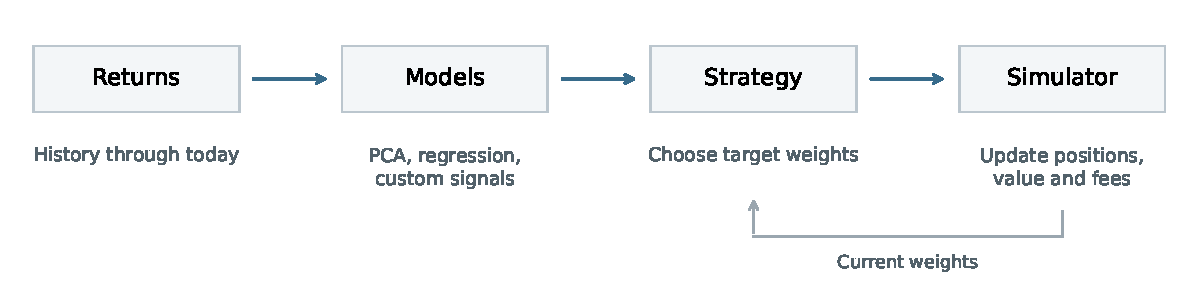
\includegraphics[width=\linewidth]{figures/framework_components.pdf}
    \caption{Daily data flow through the backtesting framework. Return
    history available through the current close enters the model sequence,
    which includes PCA, factor regression, and any custom signals.
    The strategy converts these outputs into target portfolio weights,
    while the simulator handles positions, returns, trades, and fees.
    The return arrow supplies the strategy with current weights after
    market movements, allowing it to calculate the next adjustment.
    The diagram shows one strategy, but several independent portfolios
    can use the same model outputs.}
    \label{fig:framework-components}
\end{figure}

\subsection{Rolling estimates}

Our PCA and factor models use rolling windows: fixed-length segments of
recent return history that advance as new observations arrive. Each model
has a configurable window length and refitting interval, which determine
how much history enters a fit and how often the estimate changes.
For example, a PCA model with a 500-day window and a five-day interval
fits on the latest 500 returns, reuses the estimate for four more days,
and then refits on the updated window. Because the factor regression has
its own window and interval, a strategy can estimate common factors from
a longer history while allowing stock exposures to respond more quickly
to recent observations.

At a PCA refit, we subtract each stock's mean and divide by its sample
standard deviation within that window, preventing highly volatile stocks
from dominating solely because of their larger return variation. After
retaining the leading \(K\) components, the regression converts them into
factor weights using the same volatility estimates and calculates factor
returns over its own window. Regressing each stock's returns on these
factors and an intercept then produces its estimated alpha and exposures.

To maintain a consistent factor definition within each regression, all
observations use the same active PCA weights. A new PCA estimate therefore
triggers a regression refit even before the regression's usual interval
elapses. Between refits, coefficients remain fixed while factor returns
and residuals update with each day's observations.

The same timing restriction applies to every stage of estimation,
including standardization, so future returns and volatility cannot enter
an earlier fit. Refitting also leaves earlier trading decisions unchanged.
Together, these conventions avoid look-ahead from model estimation,
although they do not eliminate the selection bias associated with
developing strategies through repeated experiments.

Custom signal models use the same daily flow, managing their own windows
and update schedules from the history of earlier outputs. When a model
learns from a five-day return, for example, that observation enters training
only after the full holding period ends. Strategies receive the updated
estimates through a common interface without changes to the simulation.

\begin{figure}[htbp]
    \centering
    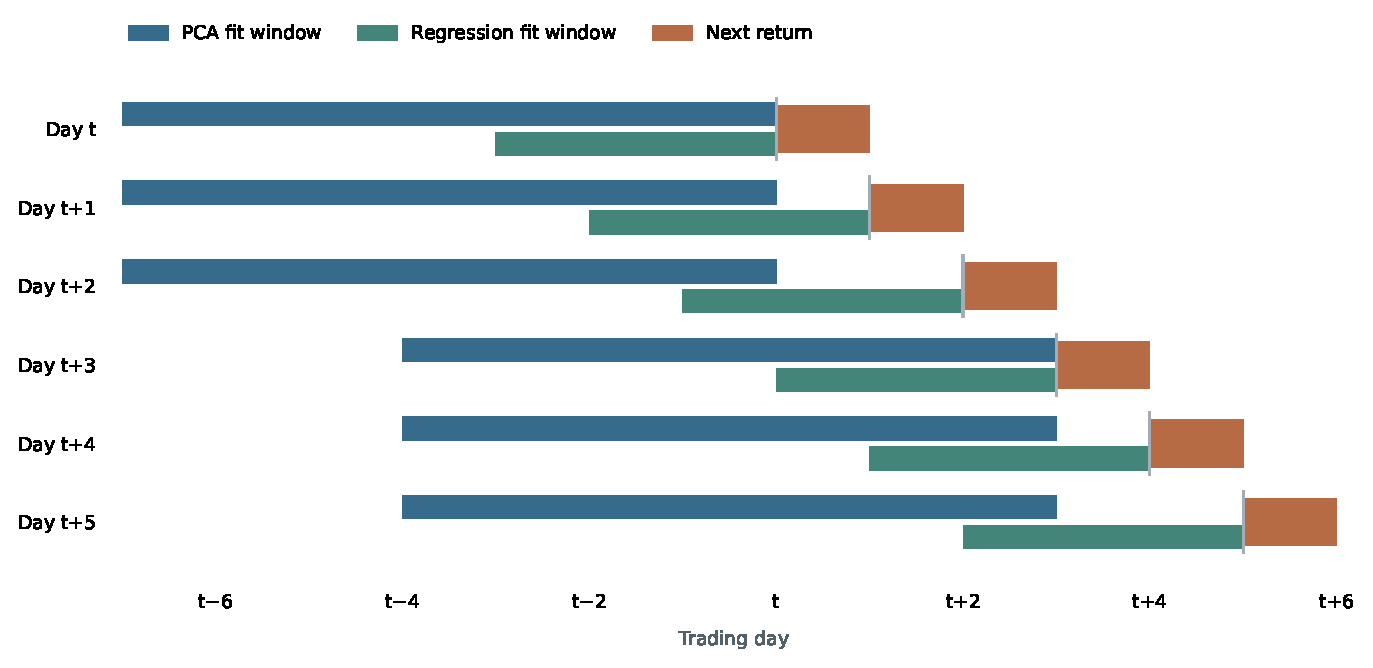
\includegraphics[width=\linewidth]{figures/framework_walkforward.pdf}
    \caption{Walk-forward estimation over six consecutive decision dates.
    Each row represents the portfolio decision at the indicated day's
    close, marked by the vertical gray line. Blue bars identify the
    observations used by the active PCA estimate, and green bars identify
    the regression window. In this example, PCA refits at \(t\) and
    \(t+3\), so its estimation window remains unchanged for three rows
    before advancing. The regression refits daily using the active PCA
    weights, including a new factor basis when PCA updates. Orange bars
    show the subsequent return interval earned by the chosen portfolio.
    Estimation periods lie entirely before or at the decision close,
    while portfolio returns occur afterward. Window lengths and the
    three-day PCA interval are illustrative rather than strategy defaults.}
    \label{fig:framework-walkforward}
\end{figure}

\subsection{Cool sidenote: PCA optimization}

Rolling PCA requires repeatedly fitting the model as the window advances,
which becomes slow when we test many parameter settings. Our basic
implementation computes all 1,201 eigenvalues and eigenvectors of the
stock covariance matrix, even when we use only five factors. We replace
this full decomposition with an iterative solver that computes only the
largest \(K\) eigenvalues and their eigenvectors. Comparing the methods
on the same return windows, we find that a 500-day fit with 1,201 stocks
and five factors takes about 264 ms with the basic method and 13.1 ms
with the optimized method, giving a median paired speedup of roughly
\(19\times\). The figures below compare runtime across different problem
sizes and show that the resulting eigenvalues and factor subspaces agree
closely. The gain is smaller for small stock universes, but it substantially
reduces the cost of repeated PCA fits on our full dataset.

\begin{figure}[htbp]
    \centering
    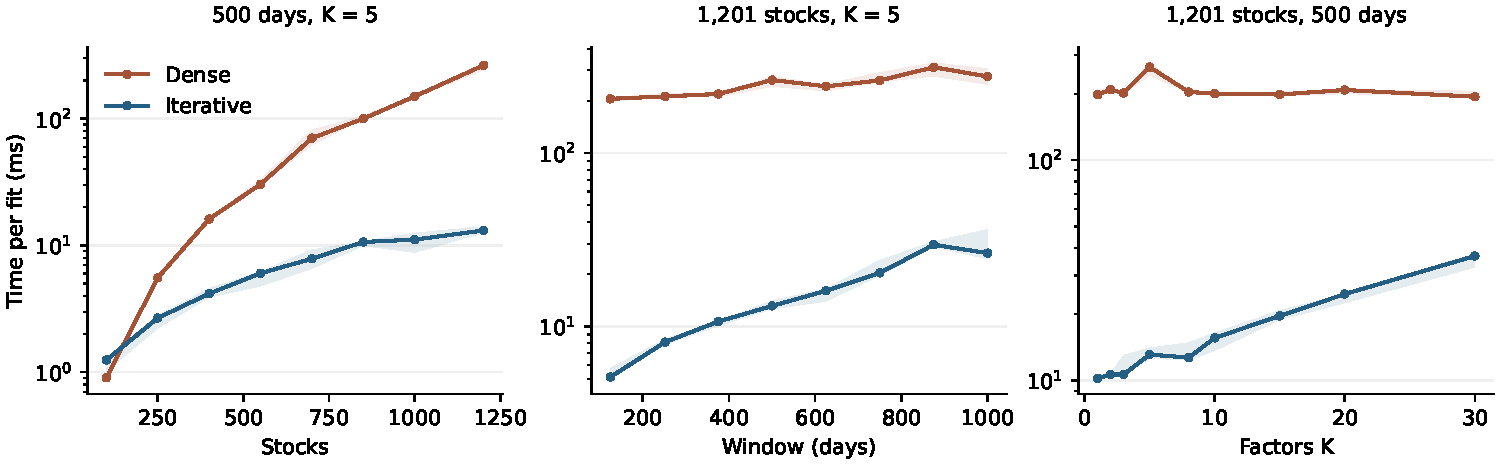
\includegraphics[width=\linewidth]{figures/pca_benchmark.pdf}
    \caption{PCA runtime as stock count, window length, and factor count
    vary, with other settings fixed as indicated above each panel.
    Points summarize the median of three window medians, each based on
    five runs. Shading spans the window medians rather than a confidence
    interval. Times include standardization and fitting, and the vertical
    axes are logarithmic. The iterative method's
    advantage grows with universe size but decreases as more factors
    are requested.}
    \label{fig:pca-benchmark}
\end{figure}

\begin{figure}[htbp]
    \centering
    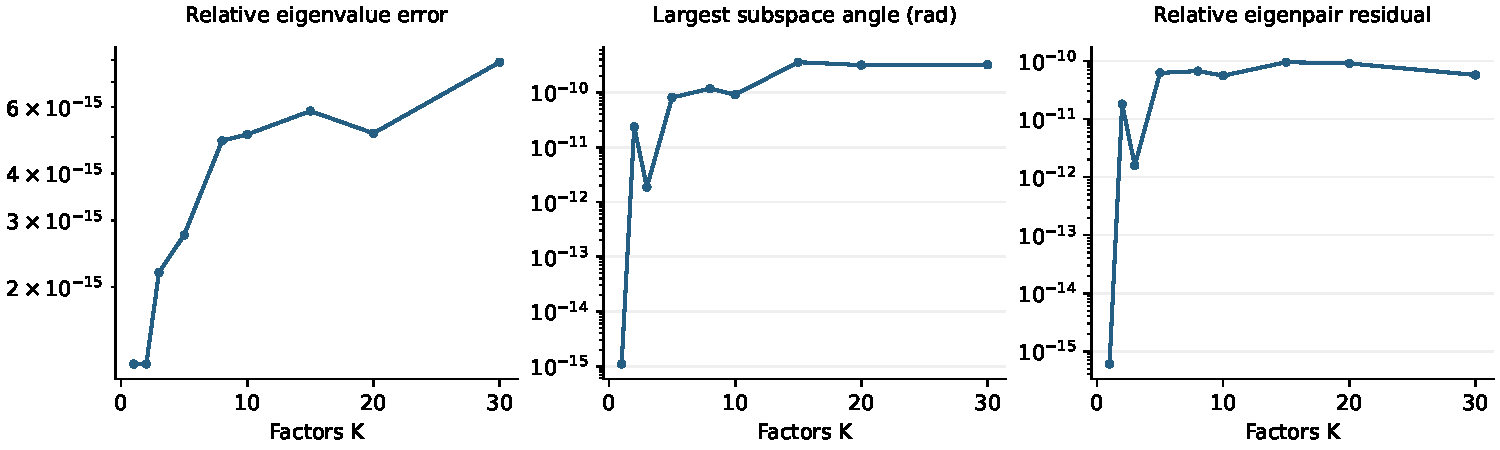
\includegraphics[width=\linewidth]{figures/pca_agreement.pdf}
    \caption{Numerical accuracy for 1,201 stocks and 500-day windows.
    The panels show relative eigenvalue differences, the largest angle
    between factor subspaces, and relative eigenpair residuals. Subspace
    angles account for arbitrary eigenvector signs, while residuals check
    the covariance eigenvalue equation directly. Each point is the worst
    value across three windows and five fits. Lower is better, and the
    logarithmic vertical axes have different scales. All checks pass
    the respective limits of \(10^{-8}\), \(10^{-6}\) radians, and
    \(10^{-8}\).}
    \label{fig:pca-agreement}
\end{figure}

\subsection{Execution and trading costs}

Our simulator applies daily returns to existing positions before executing
the next portfolio adjustment. Positions carried into day \(t\) therefore
earn that day's returns, while newly chosen weights \(w_{i,t}\) earn
returns on day \(t+1\):
\[
    r_{\mathrm{port},t+1}^{\mathrm{gross}}
    = \sum_i w_{i,t}r_{i,t+1}.
\]
Strategies hold cash until their required estimates are available, after
which we assume execution at the close used to calculate the signal.
This approximates observing prices immediately before the close and
submitting orders in time, but abstracts from processing delays and
differences between observed and executed prices. Introducing an additional
day of delay tests how strongly performance depends on immediate execution.

We calculate turnover from the weights after market movements to the new
targets, capturing the trades needed to restore an allocation even when
its target is unchanged. Positions held without adjustment incur no
rebalancing charge. The baseline deducts 5 basis points per dollar bought
or sold, including both entry and exit, while comparisons at higher fee
levels assess the sensitivity of net returns to execution costs.

\subsection{Strategy development and evaluation}

We divide evaluation into chronological training, validation, and final
holdout periods, using the training sample to develop signals and compare
candidate settings. Validation then assesses their performance on later
observations and informs the final selection. This chronological structure
preserves the order in which information becomes available, whereas a
random split would allow later market conditions to influence choices
evaluated on earlier observations.

Before the final holdout, we fix the trading rules, parameter settings,
cost assumptions, missing-data treatment, and performance measures, then
evaluate the holdout exactly once and retain the result regardless of
performance. This separates the final assessment from strategy selection.
Model estimates continue to update as observations arrive, but their
update rules remain fixed. A 500-day window, for example, continues to
advance without its length being reconsidered in response to holdout
results.

Each strategy section follows the same sequence so readers can compare
the evidence:
\begin{enumerate}
    \item \textbf{Strategy specification.} Explain the signal's motivation
    and conversion into weights, specifying estimation windows, refitting
    and trading intervals, and exposure limits.
    \item \textbf{Performance.} Report gross and net cumulative returns,
    annual results, drawdowns, and turnover to identify concentration in
    exceptional years and the contribution of trading costs.
    \item \textbf{Parameter sensitivity.} Vary nearby settings and factor
    count \(K\) over common dates after the longest warm-up. Compare
    full-sample and rolling estimates to assess how future information
    affects performance and the apparent preferred factor count.
    \item \textbf{Signal validation.} Compare subsequent returns across
    signal-strength groups and holding periods, accounting for dependence
    between overlapping returns when assessing uncertainty.
    \item \textbf{Implementation sensitivity.} Test higher fees, delayed
    execution, and exposure drift to identify dependence on low costs,
    immediate fills, or unintended risk.
    \item \textbf{Final holdout.} Report the fixed strategy's holdout result
    alongside training and validation performance, including deterioration.
\end{enumerate}

We report Sharpe ratios using daily returns, a zero risk-free-rate
convention, and annualization by \(\sqrt{252}\). For the assignment's
information ratio, we subtract fitted market exposure from portfolio
returns, divide their mean by their standard deviation, and apply the
same annualization. We state the benchmark and report market beta so
readers can see whether profits come with market exposure.

\subsection{Limitations}

Our tests address information timing, parameter sensitivity, and execution
assumptions, but the following biases and modeling limits remain relevant
when interpreting performance.

\begin{itemize}
    \item \textbf{Multiple-testing bias and validation overfitting.}
    Searching across signals and settings increases the chance of selecting
    a result that partly reflects luck. Repeated validation also makes
    those observations part of strategy selection, even when individual
    backtests use rolling estimates. Sensitivity checks and a final holdout
    strengthen the evidence without making the selected historical Sharpe
    ratio an unbiased estimate of future performance.

    \item \textbf{Survivorship and universe-selection bias.} The original
    panel contains long histories for 1,201 stocks over 2000--2023 and may
    underrepresent failed firms, delisted securities, and later entrants.
    Its selection procedure is unverified, so we cannot establish that
    the universe matches the securities available on each historical date.
    Rolling estimation restricts the information entering a fit but does
    not correct selection of the stocks themselves.

    \item \textbf{Missing-data and delisting bias.} Holdout gaps may
    coincide with illiquidity, suspensions, or corporate events rather
    than occur randomly. Dropping affected securities changes the universe,
    while assigning zero returns assumes that positions retain their value.
    We fix data-handling rules before evaluation, but incomplete terminal
    returns and public-source proxies still limit portfolio-value accuracy.

    \item \textbf{Execution and transaction-cost optimism.} Closing-price
    execution assumes negligible processing time and access to the observed
    price. Proportional fees omit market impact and stock-specific spreads,
    while the baseline also omits borrow costs and availability and assumes
    zero cash interest. These simplifications can overstate implementable
    returns. Higher-fee and delayed-execution tests assess sensitivity but
    do not establish achievable fills at a given portfolio size.

    \item \textbf{Model misspecification and exposure-estimation risk.}
    Estimated PCA exposures may omit relevant risks or change as market
    relationships evolve. Neutrality to fitted factors therefore does not
    guarantee neutrality to a market benchmark or other systematic risks.
    Position drift adds exposure between rebalances, making realized beta
    and drawdowns necessary complements to model-based neutrality.

    \item \textbf{Regime dependence and limited external validity.} The
    final holdout covers one subsequent combination of volatility, liquidity,
    and investor behavior. Annual comparisons reveal concentration in
    particular episodes, but a successful holdout does not establish
    performance under different market conditions. Conclusions therefore
    apply to the observed periods without implying stable future returns.
\end{itemize}
.

\section{Backtesting Framework and Methodology}
\label{sec:framework}

We evaluate strategies through a daily simulation that updates model
estimates from the available history, constructs portfolios, and measures
their subsequent returns. By separating these tasks within a common
framework, we can compare trading rules and model settings while keeping
the data flow and portfolio accounting consistent.

\subsection{Framework structure}

The framework separates three tasks:
\begin{itemize}
    \item \textbf{Models.} Convert return history into estimates and signals.
    \item \textbf{Strategies.} Use model outputs to choose portfolio weights.
    \item \textbf{Simulator.} Track positions, trades, fees, and portfolio value.
\end{itemize}
The daily return history first enters the PCA model, whose components
and volatility estimates feed the factor regression. The regression then
produces stock alphas, exposures, and residuals, which strategies can use
directly or pass to additional signal models.
Models run in dependency order so that each receives the estimates it
requires before producing its own output.

Each strategy receives the model outputs and its current portfolio
weights, then returns target weights for the simulator to implement.
The simulator calculates the required trades and fees, applies the next
day's returns to the resulting positions, and passes the updated weights
back to the strategy. Keeping this accounting separate from the trading
rule allows several strategies to share model estimates while maintaining
independent portfolios, reducing repeated computation and ensuring that
their decisions use comparable inputs.

\begin{figure}[htbp]
    \centering
    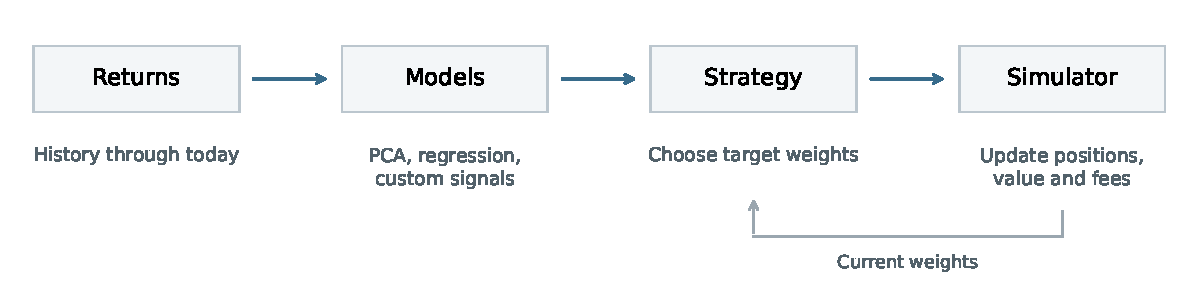
\includegraphics[width=\linewidth]{figures/framework_components.pdf}
    \caption{Daily data flow through the backtesting framework. Return
    history available through the current close enters the model sequence,
    which includes PCA, factor regression, and any custom signals.
    The strategy converts these outputs into target portfolio weights,
    while the simulator handles positions, returns, trades, and fees.
    The return arrow supplies the strategy with current weights after
    market movements, allowing it to calculate the next adjustment.
    The diagram shows one strategy, but several independent portfolios
    can use the same model outputs.}
    \label{fig:framework-components}
\end{figure}

\subsection{Rolling estimates}

Our PCA and factor models use rolling windows: fixed-length segments of
recent return history that advance as new observations arrive. Each model
has a configurable window length and refitting interval, which determine
how much history enters a fit and how often the estimate changes.
For example, a PCA model with a 500-day window and a five-day interval
fits on the latest 500 returns, reuses the estimate for four more days,
and then refits on the updated window. Because the factor regression has
its own window and interval, a strategy can estimate common factors from
a longer history while allowing stock exposures to respond more quickly
to recent observations.

At a PCA refit, we subtract each stock's mean and divide by its sample
standard deviation within that window, preventing highly volatile stocks
from dominating solely because of their larger return variation. After
retaining the leading \(K\) components, the regression converts them into
factor weights using the same volatility estimates and calculates factor
returns over its own window. Regressing each stock's returns on these
factors and an intercept then produces its estimated alpha and exposures.

To maintain a consistent factor definition within each regression, all
observations use the same active PCA weights. A new PCA estimate therefore
triggers a regression refit even before the regression's usual interval
elapses. Between refits, coefficients remain fixed while factor returns
and residuals update with each day's observations.

The same timing restriction applies to every stage of estimation,
including standardization, so future returns and volatility cannot enter
an earlier fit. Refitting also leaves earlier trading decisions unchanged.
Together, these conventions avoid look-ahead from model estimation,
although they do not eliminate the selection bias associated with
developing strategies through repeated experiments.

Custom signal models use the same daily flow, managing their own windows
and update schedules from the history of earlier outputs. When a model
learns from a five-day return, for example, that observation enters training
only after the full holding period ends. Strategies receive the updated
estimates through a common interface without changes to the simulation.

\begin{figure}[htbp]
    \centering
    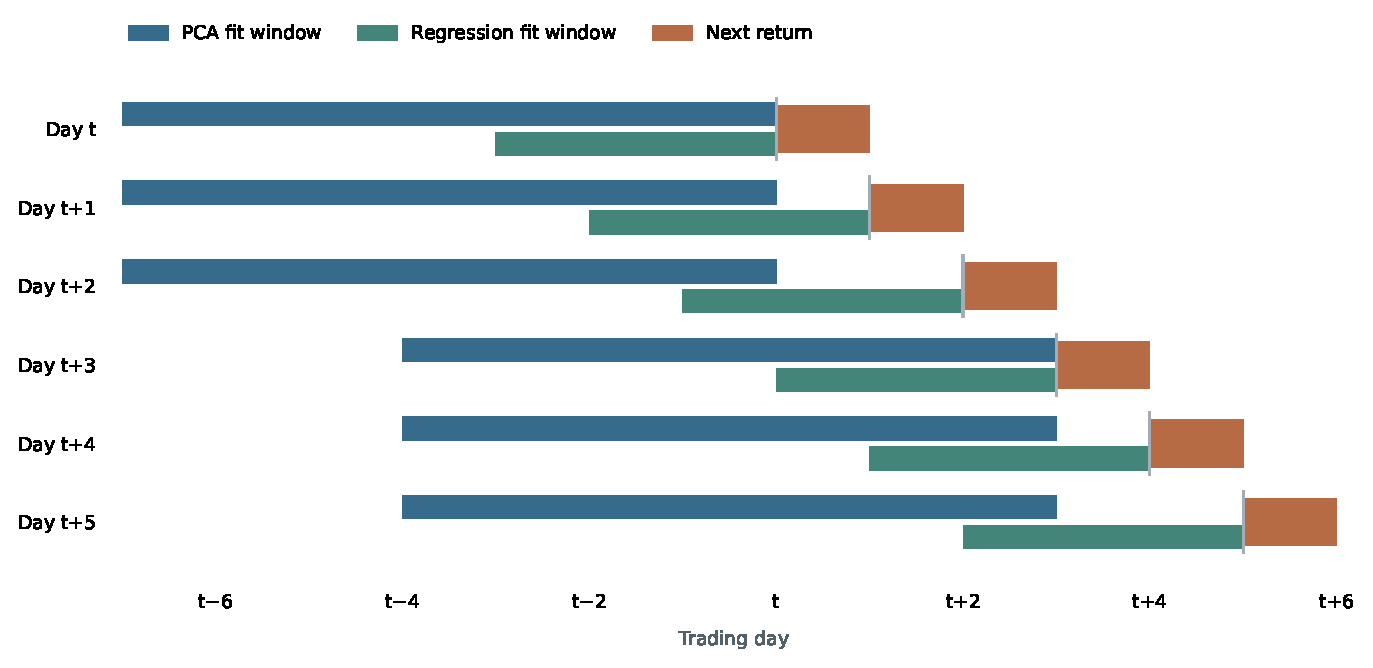
\includegraphics[width=\linewidth]{figures/framework_walkforward.pdf}
    \caption{Walk-forward estimation over six consecutive decision dates.
    Each row represents the portfolio decision at the indicated day's
    close, marked by the vertical gray line. Blue bars identify the
    observations used by the active PCA estimate, and green bars identify
    the regression window. In this example, PCA refits at \(t\) and
    \(t+3\), so its estimation window remains unchanged for three rows
    before advancing. The regression refits daily using the active PCA
    weights, including a new factor basis when PCA updates. Orange bars
    show the subsequent return interval earned by the chosen portfolio.
    Estimation periods lie entirely before or at the decision close,
    while portfolio returns occur afterward. Window lengths and the
    three-day PCA interval are illustrative rather than strategy defaults.}
    \label{fig:framework-walkforward}
\end{figure}

\subsection{Cool sidenote: PCA optimization}

Rolling PCA requires repeatedly fitting the model as the window advances,
which becomes slow when we test many parameter settings. Our basic
implementation computes all 1,201 eigenvalues and eigenvectors of the
stock covariance matrix, even when we use only five factors. We replace
this full decomposition with an iterative solver that computes only the
largest \(K\) eigenvalues and their eigenvectors. Comparing the methods
on the same return windows, we find that a 500-day fit with 1,201 stocks
and five factors takes about 264 ms with the basic method and 13.1 ms
with the optimized method, giving a median paired speedup of roughly
\(19\times\). The figures below compare runtime across different problem
sizes and show that the resulting eigenvalues and factor subspaces agree
closely. The gain is smaller for small stock universes, but it substantially
reduces the cost of repeated PCA fits on our full dataset.

\begin{figure}[htbp]
    \centering
    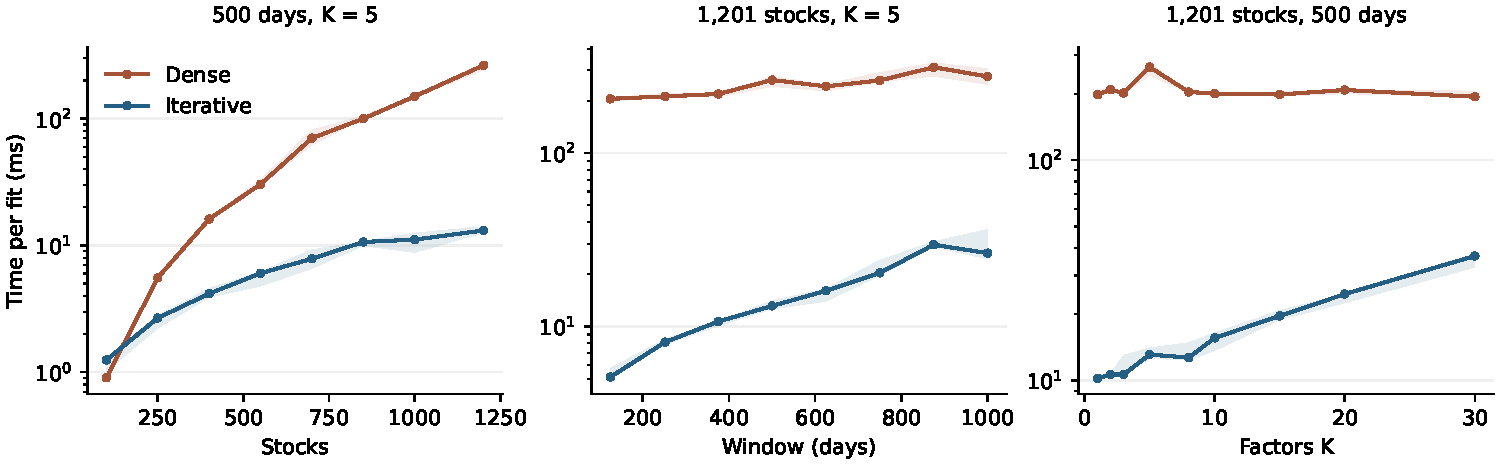
\includegraphics[width=\linewidth]{figures/pca_benchmark.pdf}
    \caption{PCA runtime as stock count, window length, and factor count
    vary, with other settings fixed as indicated above each panel.
    Points summarize the median of three window medians, each based on
    five runs. Shading spans the window medians rather than a confidence
    interval. Times include standardization and fitting, and the vertical
    axes are logarithmic. The iterative method's
    advantage grows with universe size but decreases as more factors
    are requested.}
    \label{fig:pca-benchmark}
\end{figure}

\begin{figure}[htbp]
    \centering
    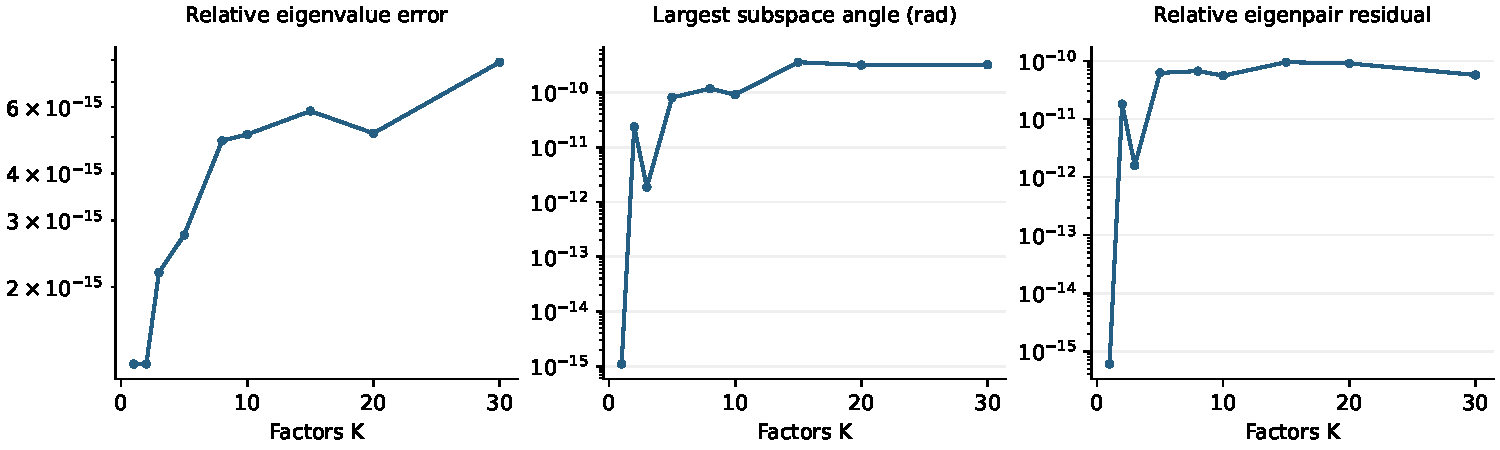
\includegraphics[width=\linewidth]{figures/pca_agreement.pdf}
    \caption{Numerical accuracy for 1,201 stocks and 500-day windows.
    The panels show relative eigenvalue differences, the largest angle
    between factor subspaces, and relative eigenpair residuals. Subspace
    angles account for arbitrary eigenvector signs, while residuals check
    the covariance eigenvalue equation directly. Each point is the worst
    value across three windows and five fits. Lower is better, and the
    logarithmic vertical axes have different scales. All checks pass
    the respective limits of \(10^{-8}\), \(10^{-6}\) radians, and
    \(10^{-8}\).}
    \label{fig:pca-agreement}
\end{figure}

\subsection{Execution and trading costs}

Our simulator applies daily returns to existing positions before executing
the next portfolio adjustment. Positions carried into day \(t\) therefore
earn that day's returns, while newly chosen weights \(w_{i,t}\) earn
returns on day \(t+1\):
\[
    r_{\mathrm{port},t+1}^{\mathrm{gross}}
    = \sum_i w_{i,t}r_{i,t+1}.
\]
Strategies hold cash until their required estimates are available, after
which we assume execution at the close used to calculate the signal.
This approximates observing prices immediately before the close and
submitting orders in time, but abstracts from processing delays and
differences between observed and executed prices. Introducing an additional
day of delay tests how strongly performance depends on immediate execution.

We calculate turnover from the weights after market movements to the new
targets, capturing the trades needed to restore an allocation even when
its target is unchanged. Positions held without adjustment incur no
rebalancing charge. The baseline deducts 5 basis points per dollar bought
or sold, including both entry and exit, while comparisons at higher fee
levels assess the sensitivity of net returns to execution costs.

\subsection{Strategy development and evaluation}

We divide evaluation into chronological training, validation, and final
holdout periods, using the training sample to develop signals and compare
candidate settings. Validation then assesses their performance on later
observations and informs the final selection. This chronological structure
preserves the order in which information becomes available, whereas a
random split would allow later market conditions to influence choices
evaluated on earlier observations.

Before the final holdout, we fix the trading rules, parameter settings,
cost assumptions, missing-data treatment, and performance measures, then
evaluate the holdout exactly once and retain the result regardless of
performance. This separates the final assessment from strategy selection.
Model estimates continue to update as observations arrive, but their
update rules remain fixed. A 500-day window, for example, continues to
advance without its length being reconsidered in response to holdout
results.

Each strategy section follows the same sequence so readers can compare
the evidence:
\begin{enumerate}
    \item \textbf{Strategy specification.} Explain the signal's motivation
    and conversion into weights, specifying estimation windows, refitting
    and trading intervals, and exposure limits.
    \item \textbf{Performance.} Report gross and net cumulative returns,
    annual results, drawdowns, and turnover to identify concentration in
    exceptional years and the contribution of trading costs.
    \item \textbf{Parameter sensitivity.} Vary nearby settings and factor
    count \(K\) over common dates after the longest warm-up. Compare
    full-sample and rolling estimates to assess how future information
    affects performance and the apparent preferred factor count.
    \item \textbf{Signal validation.} Compare subsequent returns across
    signal-strength groups and holding periods, accounting for dependence
    between overlapping returns when assessing uncertainty.
    \item \textbf{Implementation sensitivity.} Test higher fees, delayed
    execution, and exposure drift to identify dependence on low costs,
    immediate fills, or unintended risk.
    \item \textbf{Final holdout.} Report the fixed strategy's holdout result
    alongside training and validation performance, including deterioration.
\end{enumerate}

We report Sharpe ratios using daily returns, a zero risk-free-rate
convention, and annualization by \(\sqrt{252}\). For the assignment's
information ratio, we subtract fitted market exposure from portfolio
returns, divide their mean by their standard deviation, and apply the
same annualization. We state the benchmark and report market beta so
readers can see whether profits come with market exposure.

\subsection{Limitations}

Our tests address information timing, parameter sensitivity, and execution
assumptions, but the following biases and modeling limits remain relevant
when interpreting performance.

\begin{itemize}
    \item \textbf{Multiple-testing bias and validation overfitting.}
    Searching across signals and settings increases the chance of selecting
    a result that partly reflects luck. Repeated validation also makes
    those observations part of strategy selection, even when individual
    backtests use rolling estimates. Sensitivity checks and a final holdout
    strengthen the evidence without making the selected historical Sharpe
    ratio an unbiased estimate of future performance.

    \item \textbf{Survivorship and universe-selection bias.} The original
    panel contains long histories for 1,201 stocks over 2000--2023 and may
    underrepresent failed firms, delisted securities, and later entrants.
    Its selection procedure is unverified, so we cannot establish that
    the universe matches the securities available on each historical date.
    Rolling estimation restricts the information entering a fit but does
    not correct selection of the stocks themselves.

    \item \textbf{Missing-data and delisting bias.} Holdout gaps may
    coincide with illiquidity, suspensions, or corporate events rather
    than occur randomly. Dropping affected securities changes the universe,
    while assigning zero returns assumes that positions retain their value.
    We fix data-handling rules before evaluation, but incomplete terminal
    returns and public-source proxies still limit portfolio-value accuracy.

    \item \textbf{Execution and transaction-cost optimism.} Closing-price
    execution assumes negligible processing time and access to the observed
    price. Proportional fees omit market impact and stock-specific spreads,
    while the baseline also omits borrow costs and availability and assumes
    zero cash interest. These simplifications can overstate implementable
    returns. Higher-fee and delayed-execution tests assess sensitivity but
    do not establish achievable fills at a given portfolio size.

    \item \textbf{Model misspecification and exposure-estimation risk.}
    Estimated PCA exposures may omit relevant risks or change as market
    relationships evolve. Neutrality to fitted factors therefore does not
    guarantee neutrality to a market benchmark or other systematic risks.
    Position drift adds exposure between rebalances, making realized beta
    and drawdowns necessary complements to model-based neutrality.

    \item \textbf{Regime dependence and limited external validity.} The
    final holdout covers one subsequent combination of volatility, liquidity,
    and investor behavior. Annual comparisons reveal concentration in
    particular episodes, but a successful holdout does not establish
    performance under different market conditions. Conclusions therefore
    apply to the observed periods without implying stable future returns.
\end{itemize}
.

\section{Backtesting Framework and Methodology}
\label{sec:framework}

We evaluate strategies through a daily simulation that updates model
estimates from the available history, constructs portfolios, and measures
their subsequent returns. By separating these tasks within a common
framework, we can compare trading rules and model settings while keeping
the data flow and portfolio accounting consistent.

\subsection{Framework structure}

The framework separates three tasks:
\begin{itemize}
    \item \textbf{Models.} Convert return history into estimates and signals.
    \item \textbf{Strategies.} Use model outputs to choose portfolio weights.
    \item \textbf{Simulator.} Track positions, trades, fees, and portfolio value.
\end{itemize}
The daily return history first enters the PCA model, whose components
and volatility estimates feed the factor regression. The regression then
produces stock alphas, exposures, and residuals, which strategies can use
directly or pass to additional signal models.
Models run in dependency order so that each receives the estimates it
requires before producing its own output.

Each strategy receives the model outputs and its current portfolio
weights, then returns target weights for the simulator to implement.
The simulator calculates the required trades and fees, applies the next
day's returns to the resulting positions, and passes the updated weights
back to the strategy. Keeping this accounting separate from the trading
rule allows several strategies to share model estimates while maintaining
independent portfolios, reducing repeated computation and ensuring that
their decisions use comparable inputs.

\begin{figure}[htbp]
    \centering
    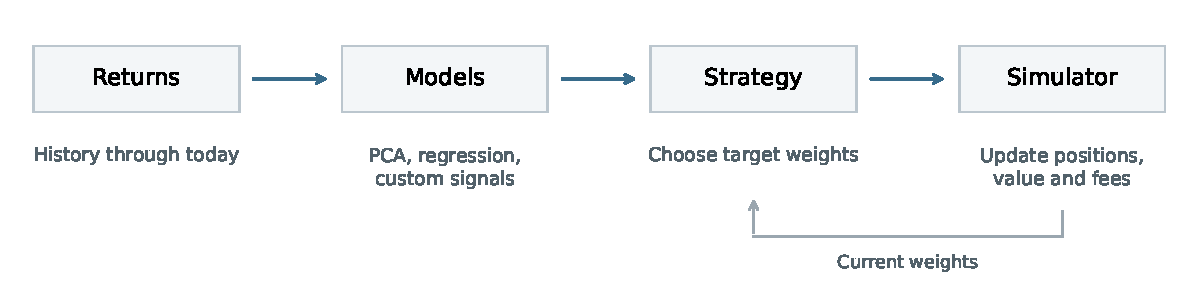
\includegraphics[width=\linewidth]{figures/framework_components.pdf}
    \caption{Daily data flow through the backtesting framework. Return
    history available through the current close enters the model sequence,
    which includes PCA, factor regression, and any custom signals.
    The strategy converts these outputs into target portfolio weights,
    while the simulator handles positions, returns, trades, and fees.
    The return arrow supplies the strategy with current weights after
    market movements, allowing it to calculate the next adjustment.
    The diagram shows one strategy, but several independent portfolios
    can use the same model outputs.}
    \label{fig:framework-components}
\end{figure}

\subsection{Rolling estimates}

Our PCA and factor models use rolling windows: fixed-length segments of
recent return history that advance as new observations arrive. Each model
has a configurable window length and refitting interval, which determine
how much history enters a fit and how often the estimate changes.
For example, a PCA model with a 500-day window and a five-day interval
fits on the latest 500 returns, reuses the estimate for four more days,
and then refits on the updated window. Because the factor regression has
its own window and interval, a strategy can estimate common factors from
a longer history while allowing stock exposures to respond more quickly
to recent observations.

At a PCA refit, we subtract each stock's mean and divide by its sample
standard deviation within that window, preventing highly volatile stocks
from dominating solely because of their larger return variation. After
retaining the leading \(K\) components, the regression converts them into
factor weights using the same volatility estimates and calculates factor
returns over its own window. Regressing each stock's returns on these
factors and an intercept then produces its estimated alpha and exposures.

To maintain a consistent factor definition within each regression, all
observations use the same active PCA weights. A new PCA estimate therefore
triggers a regression refit even before the regression's usual interval
elapses. Between refits, coefficients remain fixed while factor returns
and residuals update with each day's observations.

The same timing restriction applies to every stage of estimation,
including standardization, so future returns and volatility cannot enter
an earlier fit. Refitting also leaves earlier trading decisions unchanged.
Together, these conventions avoid look-ahead from model estimation,
although they do not eliminate the selection bias associated with
developing strategies through repeated experiments.

Custom signal models use the same daily flow, managing their own windows
and update schedules from the history of earlier outputs. When a model
learns from a five-day return, for example, that observation enters training
only after the full holding period ends. Strategies receive the updated
estimates through a common interface without changes to the simulation.

\begin{figure}[htbp]
    \centering
    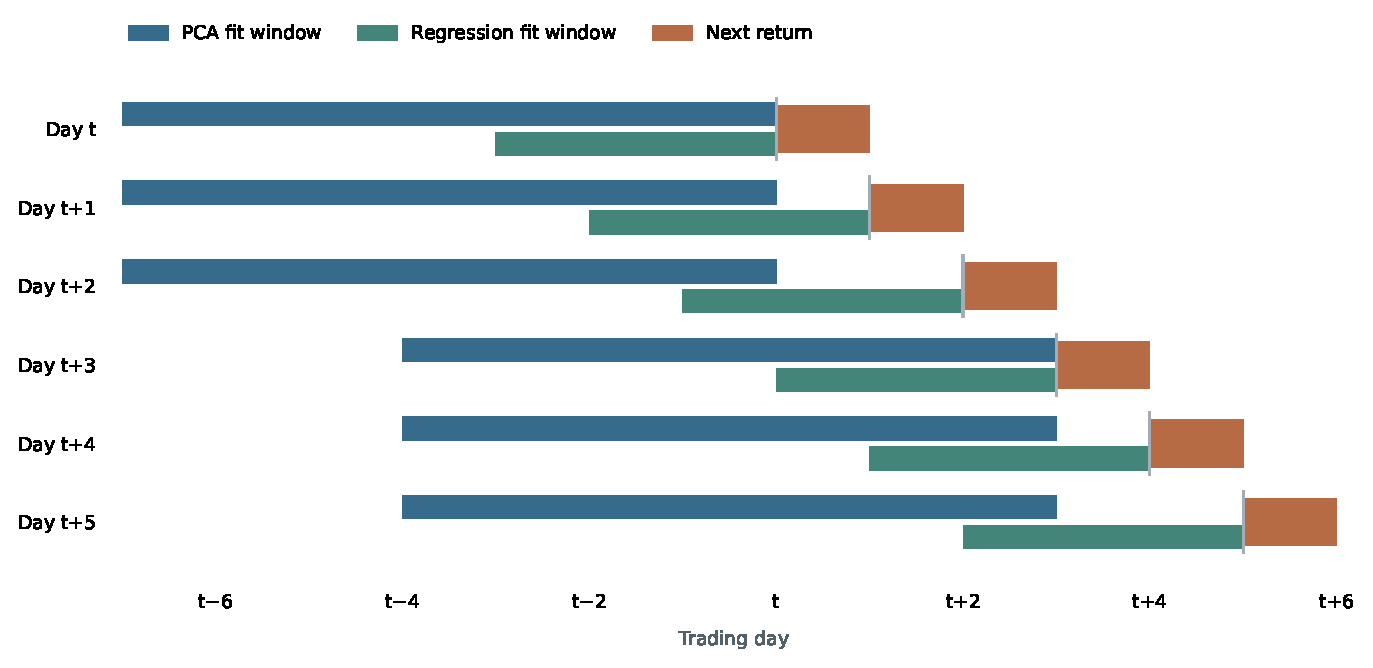
\includegraphics[width=\linewidth]{figures/framework_walkforward.pdf}
    \caption{Walk-forward estimation over six consecutive decision dates.
    Each row represents the portfolio decision at the indicated day's
    close, marked by the vertical gray line. Blue bars identify the
    observations used by the active PCA estimate, and green bars identify
    the regression window. In this example, PCA refits at \(t\) and
    \(t+3\), so its estimation window remains unchanged for three rows
    before advancing. The regression refits daily using the active PCA
    weights, including a new factor basis when PCA updates. Orange bars
    show the subsequent return interval earned by the chosen portfolio.
    Estimation periods lie entirely before or at the decision close,
    while portfolio returns occur afterward. Window lengths and the
    three-day PCA interval are illustrative rather than strategy defaults.}
    \label{fig:framework-walkforward}
\end{figure}

\subsection{Cool sidenote: PCA optimization}

Rolling PCA requires repeatedly fitting the model as the window advances,
which becomes slow when we test many parameter settings. Our basic
implementation computes all 1,201 eigenvalues and eigenvectors of the
stock covariance matrix, even when we use only five factors. We replace
this full decomposition with an iterative solver that computes only the
largest \(K\) eigenvalues and their eigenvectors. Comparing the methods
on the same return windows, we find that a 500-day fit with 1,201 stocks
and five factors takes about 264 ms with the basic method and 13.1 ms
with the optimized method, giving a median paired speedup of roughly
\(19\times\). The figures below compare runtime across different problem
sizes and show that the resulting eigenvalues and factor subspaces agree
closely. The gain is smaller for small stock universes, but it substantially
reduces the cost of repeated PCA fits on our full dataset.

\begin{figure}[htbp]
    \centering
    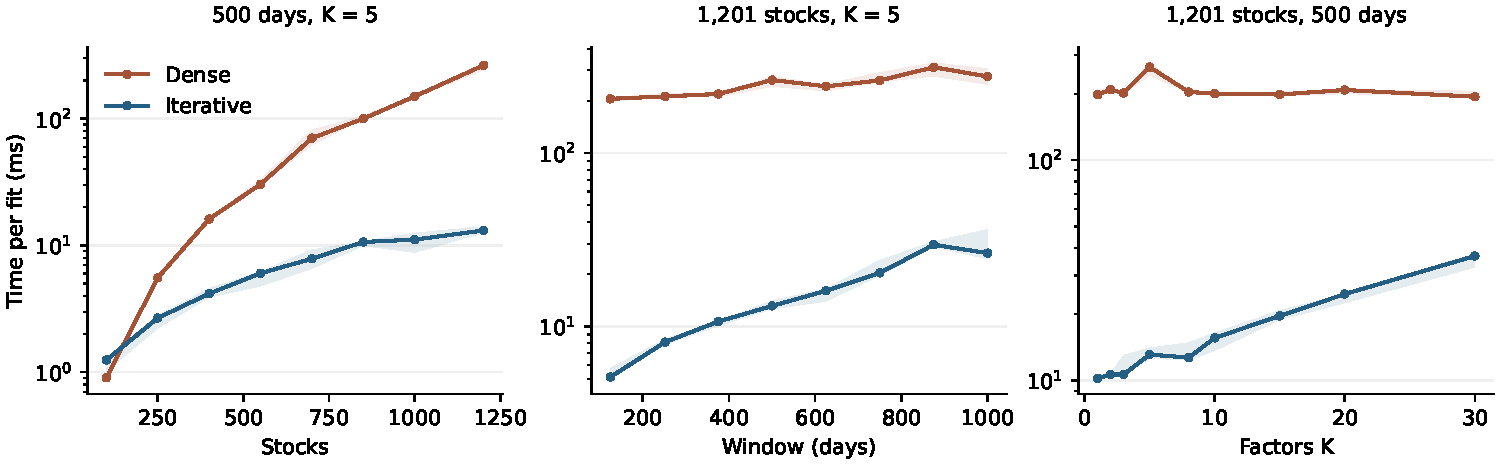
\includegraphics[width=\linewidth]{figures/pca_benchmark.pdf}
    \caption{PCA runtime as stock count, window length, and factor count
    vary, with other settings fixed as indicated above each panel.
    Points summarize the median of three window medians, each based on
    five runs. Shading spans the window medians rather than a confidence
    interval. Times include standardization and fitting, and the vertical
    axes are logarithmic. The iterative method's
    advantage grows with universe size but decreases as more factors
    are requested.}
    \label{fig:pca-benchmark}
\end{figure}

\begin{figure}[htbp]
    \centering
    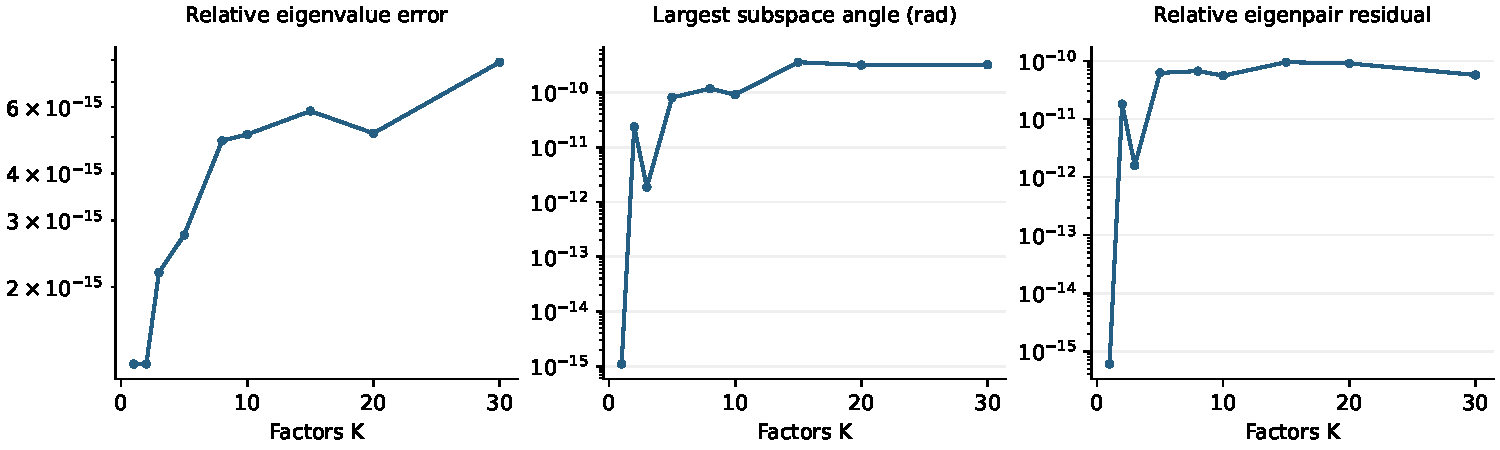
\includegraphics[width=\linewidth]{figures/pca_agreement.pdf}
    \caption{Numerical accuracy for 1,201 stocks and 500-day windows.
    The panels show relative eigenvalue differences, the largest angle
    between factor subspaces, and relative eigenpair residuals. Subspace
    angles account for arbitrary eigenvector signs, while residuals check
    the covariance eigenvalue equation directly. Each point is the worst
    value across three windows and five fits. Lower is better, and the
    logarithmic vertical axes have different scales. All checks pass
    the respective limits of \(10^{-8}\), \(10^{-6}\) radians, and
    \(10^{-8}\).}
    \label{fig:pca-agreement}
\end{figure}

\subsection{Execution and trading costs}

Our simulator applies daily returns to existing positions before executing
the next portfolio adjustment. Positions carried into day \(t\) therefore
earn that day's returns, while newly chosen weights \(w_{i,t}\) earn
returns on day \(t+1\):
\[
    r_{\mathrm{port},t+1}^{\mathrm{gross}}
    = \sum_i w_{i,t}r_{i,t+1}.
\]
Strategies hold cash until their required estimates are available, after
which we assume execution at the close used to calculate the signal.
This approximates observing prices immediately before the close and
submitting orders in time, but abstracts from processing delays and
differences between observed and executed prices. Introducing an additional
day of delay tests how strongly performance depends on immediate execution.

We calculate turnover from the weights after market movements to the new
targets, capturing the trades needed to restore an allocation even when
its target is unchanged. Positions held without adjustment incur no
rebalancing charge. The baseline deducts 5 basis points per dollar bought
or sold, including both entry and exit, while comparisons at higher fee
levels assess the sensitivity of net returns to execution costs.

\subsection{Strategy development and evaluation}

We divide evaluation into chronological training, validation, and final
holdout periods, using the training sample to develop signals and compare
candidate settings. Validation then assesses their performance on later
observations and informs the final selection. This chronological structure
preserves the order in which information becomes available, whereas a
random split would allow later market conditions to influence choices
evaluated on earlier observations.

Before the final holdout, we fix the trading rules, parameter settings,
cost assumptions, missing-data treatment, and performance measures, then
evaluate the holdout exactly once and retain the result regardless of
performance. This separates the final assessment from strategy selection.
Model estimates continue to update as observations arrive, but their
update rules remain fixed. A 500-day window, for example, continues to
advance without its length being reconsidered in response to holdout
results.

Each strategy section follows the same sequence so readers can compare
the evidence:
\begin{enumerate}
    \item \textbf{Strategy specification.} Explain the signal's motivation
    and conversion into weights, specifying estimation windows, refitting
    and trading intervals, and exposure limits.
    \item \textbf{Performance.} Report gross and net cumulative returns,
    annual results, drawdowns, and turnover to identify concentration in
    exceptional years and the contribution of trading costs.
    \item \textbf{Parameter sensitivity.} Vary nearby settings and factor
    count \(K\) over common dates after the longest warm-up. Compare
    full-sample and rolling estimates to assess how future information
    affects performance and the apparent preferred factor count.
    \item \textbf{Signal validation.} Compare subsequent returns across
    signal-strength groups and holding periods, accounting for dependence
    between overlapping returns when assessing uncertainty.
    \item \textbf{Implementation sensitivity.} Test higher fees, delayed
    execution, and exposure drift to identify dependence on low costs,
    immediate fills, or unintended risk.
    \item \textbf{Final holdout.} Report the fixed strategy's holdout result
    alongside training and validation performance, including deterioration.
\end{enumerate}

We report Sharpe ratios using daily returns, a zero risk-free-rate
convention, and annualization by \(\sqrt{252}\). For the assignment's
information ratio, we subtract fitted market exposure from portfolio
returns, divide their mean by their standard deviation, and apply the
same annualization. We state the benchmark and report market beta so
readers can see whether profits come with market exposure.

\subsection{Limitations}

Our tests address information timing, parameter sensitivity, and execution
assumptions, but the following biases and modeling limits remain relevant
when interpreting performance.

\begin{itemize}
    \item \textbf{Multiple-testing bias and validation overfitting.}
    Searching across signals and settings increases the chance of selecting
    a result that partly reflects luck. Repeated validation also makes
    those observations part of strategy selection, even when individual
    backtests use rolling estimates. Sensitivity checks and a final holdout
    strengthen the evidence without making the selected historical Sharpe
    ratio an unbiased estimate of future performance.

    \item \textbf{Survivorship and universe-selection bias.} The original
    panel contains long histories for 1,201 stocks over 2000--2023 and may
    underrepresent failed firms, delisted securities, and later entrants.
    Its selection procedure is unverified, so we cannot establish that
    the universe matches the securities available on each historical date.
    Rolling estimation restricts the information entering a fit but does
    not correct selection of the stocks themselves.

    \item \textbf{Missing-data and delisting bias.} Holdout gaps may
    coincide with illiquidity, suspensions, or corporate events rather
    than occur randomly. Dropping affected securities changes the universe,
    while assigning zero returns assumes that positions retain their value.
    We fix data-handling rules before evaluation, but incomplete terminal
    returns and public-source proxies still limit portfolio-value accuracy.

    \item \textbf{Execution and transaction-cost optimism.} Closing-price
    execution assumes negligible processing time and access to the observed
    price. Proportional fees omit market impact and stock-specific spreads,
    while the baseline also omits borrow costs and availability and assumes
    zero cash interest. These simplifications can overstate implementable
    returns. Higher-fee and delayed-execution tests assess sensitivity but
    do not establish achievable fills at a given portfolio size.

    \item \textbf{Model misspecification and exposure-estimation risk.}
    Estimated PCA exposures may omit relevant risks or change as market
    relationships evolve. Neutrality to fitted factors therefore does not
    guarantee neutrality to a market benchmark or other systematic risks.
    Position drift adds exposure between rebalances, making realized beta
    and drawdowns necessary complements to model-based neutrality.

    \item \textbf{Regime dependence and limited external validity.} The
    final holdout covers one subsequent combination of volatility, liquidity,
    and investor behavior. Annual comparisons reveal concentration in
    particular episodes, but a successful holdout does not establish
    performance under different market conditions. Conclusions therefore
    apply to the observed periods without implying stable future returns.
\end{itemize}


\section{Trading Strategies}

We build two strategies on top of the PCA factor model. The main strategy, a \emph{contrarian factor-neutral Treynor--Black portfolio}, trades directly on the estimated alphas $\alpha_i$. The second, \emph{PCA pairs trading}, uses the principal component loadings to find pairs of economically similar stocks and trades the convergence of their prices.

The data are daily returns for $N = 1{,}201$ stocks from January 2000 to December 2023. Both strategies are simulated out-of-sample: every estimate is recomputed on a trailing window as the simulation moves forward, and trading begins in January 2002 once 500 days of history are available.

\subsection{Rolling factor model}

\begin{itemize}
    \item \textbf{Principal components.} Every 5 trading days, we run PCA on the correlation matrix of the previous 500 days of returns. Standardizing returns first prevents high-volatility stocks from dominating the components. We keep the top $K = 5$ eigenvectors $v_1, \dots, v_5$.
    \item \textbf{Factor returns.} Each eigenvector defines an eigenportfolio with return $f^k_t = \sum_i \frac{v_k[i]}{\bar\sigma_i} r_{i,t}$.
    \item \textbf{Alphas and betas.} Each day, for each stock, we regress the previous 250 days of returns on the five factor returns,
    \[
        r_{i,t} = \alpha_i + \sum_{k=1}^{K} \beta_{k,i} f^k_t + \epsilon_{i,t},
    \]
    which gives the alpha $\alpha_i$, the factor betas $\beta_{k,i}$, and the residual variance $\sigma^2(\epsilon_i)$.
\end{itemize}

\subsection{Strategy 1: Contrarian factor-neutral Treynor--Black}

\paragraph{Scores.} Under the Treynor--Black model, the optimal active weight on a stock is proportional to its alpha divided by its idiosyncratic variance: a large alpha on a very noisy stock deserves less weight than a moderate alpha on a stable one. We use the negative of this ratio,
\[
    s_i = -\frac{\alpha_i}{\sigma^2(\epsilon_i)}.
\]
The sign is flipped because, out of sample, stocks with high estimated alpha go on to \emph{underperform} (Table~\ref{tab:development}). Past alpha in this universe reverses: it reflects temporary mispricing or estimation noise, not persistent outperformance. Section~\ref{sec:holdout} confirms that this reversal is already present using only 2002--2017 data. To keep a few extreme stocks from dominating, we convert the scores to cross-sectional z-scores and cap them at $\pm 3$.

\paragraph{Factor neutrality.} We project the scores onto the space orthogonal to a vector of ones and the $K$ beta vectors, so the portfolio satisfies
\[
    \sum_i w_i = 0 \quad \text{(dollar neutral)}, \qquad \sum_i w_i \beta_{k,i} = 0 \quad \text{for } k = 1, \dots, K \quad \text{(factor neutral)}.
\]
Because the first principal component is essentially the market, this also makes the strategy approximately market neutral.

\paragraph{Scaling and trading.} Weights are scaled so gross exposure is $\sum_i |w_i| = 1$ (50\% long, 50\% short), and the portfolio is rebalanced daily.

\begin{table}[H]
\centering
\caption{Development of the strategy (out-of-sample, 2002--2023, 5bp fees unless stated).}
\label{tab:development}
\begin{tabular}{lrrrr}
\toprule
Strategy & Sharpe & Sharpe (no fees) & Return & Market beta \\
\midrule
Long top 20\% $\alpha$, short bottom 20\% & $-1.31$ & $-0.98$ & $-6.1\%$ & $-0.07$ \\
Contrarian 20\% sort & 0.66 & 0.98 & 3.1\% & 0.07 \\
Contrarian 20\% sort, factor-hedged & 0.72 & 1.12 & 2.9\% & 0.04 \\
Contrarian Treynor--Black, not hedged & 0.76 & 1.18 & 2.4\% & 0.07 \\
\textbf{Contrarian Treynor--Black, factor-hedged} & \textbf{0.85} & \textbf{1.31} & 2.5\% & 0.04 \\
\bottomrule
\end{tabular}
\end{table}

Each design choice helps. Reversing the sign turns a losing strategy into a profitable one. Weighting by $\alpha_i / \sigma^2(\epsilon_i)$ improves on equal weights. The factor hedge leaves the return almost unchanged (2.5\% vs.\ 2.4\%) but lowers volatility from 3.2\% to 2.9\% and market beta from 0.07 to 0.04: it removes unrewarded factor risk without sacrificing alpha. Market beta is measured against an equal-weighted average of all stocks in the universe.

\begin{figure}[H]
\centering
\includegraphics[width=\textwidth]{figures/cumulative_returns_tb.pdf}
\caption{Growth of \$1 invested in Contrarian Treynor--Black, with and without 5bp transaction costs. Shaded regions mark the 2008--09 financial crisis and the 2020 COVID crash.}
\label{fig:cumulative-tb}
\end{figure}

\begin{figure}[H]
\centering
\includegraphics[width=\textwidth]{figures/cumulative_returns_pairs.pdf}
\caption{Growth of \$1 invested in PCA pairs trading, with and without 5bp transaction costs. Shaded regions mark the 2008--09 financial crisis and the 2020 COVID crash.}
\label{fig:cumulative-pairs}
\end{figure}

\subsection{Strategy 2: PCA pairs trading}

\paragraph{Pair selection.} Every 21 trading days, we describe each stock by its loadings on the $K$ principal components, $\ell_i = (v_1[i]\sqrt{\lambda_1}, \dots, v_K[i]\sqrt{\lambda_K})$. We then greedily match the closest stocks in this space, keeping the 50 best non-overlapping pairs. Because the two stocks in a pair have nearly identical factor exposure, the spread between them is approximately factor neutral and driven mostly by stock-specific news.

\paragraph{Trading rule.} For each pair $(i, j)$, we track the log price ratio $\log(P_i / P_j)$ over the previous 60 days and compute its z-score $z$. When $z < -2$ we buy $i$ and short $j$; when $z > 2$ we do the reverse. We close the position once $|z| < 0.5$. Each pair is allocated a fixed $1/50$ of capital, so idle pairs hold cash.

Even though no industry data is used, the selected pairs are economically sensible: utilities (WEC/DUK, ATO/NI), natural gas producers (EQT/CNX), tower REITs (AMT/SBAC) and apartment REITs (EQR/MAA). The principal components recover industry structure from returns alone.

\subsection{Backtest design}

\paragraph{Timing and look-ahead bias.} Weights chosen at the close of day $t$ use only returns up to and including day $t$, and they earn the returns of day $t+1$: $r_{\text{port},t+1} = \sum_i w_{i,t} r_{i,t+1}$. We verified this directly: re-running the backtest on data truncated at December 2011 leaves every earlier position unchanged, up to floating-point rounding of order $10^{-13}$.

\paragraph{Transaction costs.} The assignment defines returns without costs, so we report results both without fees and with a cost of 5 basis points per dollar traded.

\paragraph{Survivorship bias.} Every stock in the sample trades continuously from 2000 to 2023, so the universe consists of firms that survived the full period. Firms that failed or were acquired are missing. This likely flatters both strategies, since buying a stock after a fall never ends in a delisting in this sample. It is a limitation of the data, not of the strategy code.

\section{Strategy Testing}

We test both strategies along six dimensions. Unless stated otherwise, all results are out-of-sample, from January 2002 to December 2023.

\subsection{Regime robustness}

\begin{table}[H]
\centering
\caption{Annual returns and Sharpe ratios.}
\label{tab:yearly}
\begin{tabular}{lrrrrrr}
\toprule
& \multicolumn{3}{c}{Contrarian Treynor--Black} & \multicolumn{3}{c}{PCA pairs trading} \\
\cmidrule(lr){2-4} \cmidrule(lr){5-7}
Year & Return & Return (5bp) & Sharpe & Return & Return (5bp) & Sharpe \\
\midrule
2002 & 5.6\% & 4.2\% & 1.93 & 13.8\% & 13.0\% & 3.52 \\
2003 & 3.6\% & 2.2\% & 1.64 & 0.9\% & 0.1\% & 0.33 \\
2004 & 2.6\% & 1.2\% & 1.51 & 2.6\% & 1.9\% & 1.02 \\
2005 & 0.7\% & $-0.7\%$ & 0.40 & 1.4\% & 0.7\% & 0.69 \\
2006 & 2.4\% & 1.1\% & 1.29 & 1.6\% & 0.8\% & 0.85 \\
2007 & $-1.1\%$ & $-2.4\%$ & $-0.38$ & 4.8\% & 4.0\% & 1.77 \\
2008 & 15.6\% & 13.7\% & 3.00 & 7.2\% & 6.2\% & 1.53 \\
2009 & 23.4\% & 21.5\% & 4.83 & 5.5\% & 4.8\% & 2.02 \\
2010 & 2.2\% & 0.8\% & 1.14 & 4.8\% & 4.1\% & 2.49 \\
2011 & 2.3\% & 0.8\% & 0.90 & 2.1\% & 1.3\% & 1.12 \\
2012 & 5.3\% & 3.9\% & 2.58 & $-0.6\%$ & $-1.2\%$ & $-0.42$ \\
2013 & 0.2\% & $-1.1\%$ & 0.14 & 1.8\% & 1.1\% & 0.94 \\
2014 & 2.7\% & 1.3\% & 1.62 & 1.1\% & 0.4\% & 0.79 \\
2015 & $-0.3\%$ & $-1.6\%$ & $-0.14$ & 0.1\% & $-0.6\%$ & 0.07 \\
2016 & 5.5\% & 4.1\% & 2.50 & 7.8\% & 7.0\% & 3.80 \\
2017 & 0.3\% & $-0.9\%$ & 0.14 & 3.9\% & 3.2\% & 2.28 \\
2018 & 1.7\% & 0.4\% & 0.70 & 3.6\% & 2.8\% & 2.06 \\
2019 & 5.1\% & 3.7\% & 2.46 & 4.5\% & 3.9\% & 2.71 \\
2020 & 8.1\% & 6.5\% & 1.26 & 9.5\% & 8.6\% & 1.91 \\
2021 & 1.6\% & 0.1\% & 0.61 & 2.7\% & 2.1\% & 1.14 \\
2022 & 1.6\% & 0.2\% & 0.44 & 0.7\% & $-0.1\%$ & 0.32 \\
2023 & $-0.8\%$ & $-2.1\%$ & $-0.22$ & 2.2\% & 1.6\% & 1.05 \\
\bottomrule
\end{tabular}
\\[4pt]
\small Returns and Sharpe ratios are without fees unless marked 5bp.
\end{table}

\begin{table}[H]
\centering
\caption{Concentration and stability of returns.}
\label{tab:regime}
\begin{tabular}{lcc}
\toprule
Measure & Treynor--Black & Pairs trading \\
\midrule
Years positive (no fees / 5bp) & 19 / 16 of 22 & 21 / 19 of 22 \\
Share of total profit from best year & 25\% (2009) & 16\% (2002) \\
Share of total profit from best two years & 43\% (2008--09) & 28\% (2002, 2020) \\
Sharpe, all years (no fees / 5bp) & 1.31 / 0.85 & 1.45 / 1.17 \\
Sharpe excluding best two years (no fees / 5bp) & 0.91 / 0.41 & 1.28 / 0.97 \\
Sharpe 2002--2012 / 2013--2023 (5bp) & 1.41 / 0.32 & 1.18 / 1.16 \\
Maximum drawdown (no fees / 5bp) & $-5.2\%$ / $-6.1\%$ & $-3.6\%$ / $-3.9\%$ \\
\bottomrule
\end{tabular}
\end{table}

No single year carries either strategy, but the two differ markedly (Figures~\ref{fig:cumulative-tb}--\ref{fig:annual-pairs}). Treynor--Black earns its best returns in crises: in 2008 it gained 15.6\% while the market fell 27\%, followed by 23.4\% in 2009 and 8.1\% in 2020. These are periods of panic selling and overreaction, when betting on reversal should pay. However, 2008--09 account for 43\% of its total profit, and its Sharpe ratio after fees fell from 1.41 in 2002--2012 to 0.32 in 2013--2023. Pairs trading is far more stable: profitable in 21 of 22 years, no more than 28\% of profit from any two years, and an essentially identical Sharpe ratio in both halves of the sample.

\begin{figure}[H]
\centering
\includegraphics[width=\textwidth]{figures/annual_returns_tb.pdf}
\caption{Annual returns of Contrarian Treynor--Black (no fees).}
\label{fig:annual-tb}
\end{figure}

\begin{figure}[H]
\centering
\includegraphics[width=\textwidth]{figures/annual_returns_pairs.pdf}
\caption{Annual returns of PCA pairs trading (no fees).}
\label{fig:annual-pairs}
\end{figure}

\subsection{Parameter sensitivity}

We vary one parameter at a time around the defaults. Because a 1000-day PCA window needs four years of history, all variants are compared over the common period beginning December 2003. The last two columns split this period into a selection period (through 2017) and a holdout period (2018--2023); see Section~\ref{sec:holdout}.

\begin{table}[H]
\centering
\caption{Parameter sensitivity: contrarian Treynor--Black.}
\label{tab:sensitivity-tb}
\begin{tabular}{llrrrrr}
\toprule
Parameter & Value & Sharpe & Sharpe (5bp) & Return (5bp) & Selection & Holdout \\
\midrule
Default & --- & 1.27 & 0.81 & 2.4\% & 1.08 & 0.40 \\
Alpha window (days) & 60 & 1.93 & 1.00 & 2.8\% & 1.13 & 0.83 \\
& 125 & 1.55 & 0.93 & 2.7\% & 1.13 & 0.64 \\
& 500 & 1.15 & 0.79 & 2.2\% & 0.88 & 0.64 \\
PCA window (days) & 250 & 1.25 & 0.78 & 2.3\% & 1.06 & 0.37 \\
& 1000 & 1.17 & 0.72 & 2.1\% & 0.96 & 0.36 \\
Score cap & 2 & 1.27 & 0.81 & 2.4\% & 1.10 & 0.39 \\
& 5 & 1.27 & 0.80 & 2.3\% & 1.06 & 0.41 \\
\bottomrule
\end{tabular}
\\[4pt]
\small Defaults: alpha window 250 days, PCA window 500 days, score cap 3. Selection and holdout columns include 5bp fees.
\end{table}

\begin{table}[H]
\centering
\caption{Parameter sensitivity: PCA pairs trading.}
\label{tab:sensitivity-pairs}
\begin{tabular}{llrrrrr}
\toprule
Parameter & Value & Sharpe & Sharpe (5bp) & Return (5bp) & Selection & Holdout \\
\midrule
Default & --- & 1.36 & 1.07 & 2.6\% & 1.04 & 1.15 \\
Entry threshold $|z|$ & 1.5 & 1.59 & 1.21 & 3.4\% & 1.20 & 1.25 \\
& 2.5 & 1.21 & 1.01 & 2.0\% & 0.92 & 1.19 \\
& 3 & 1.15 & 1.03 & 1.5\% & 0.99 & 1.14 \\
Exit threshold $|z|$ & 0 & 1.25 & 0.98 & 2.5\% & 0.97 & 1.02 \\
& 1 & 1.49 & 1.15 & 2.6\% & 1.05 & 1.37 \\
Spread window (days) & 20 & 1.93 & 1.43 & 3.4\% & 1.63 & 1.05 \\
& 40 & 1.59 & 1.25 & 3.1\% & 1.27 & 1.20 \\
& 120 & 1.29 & 1.08 & 2.6\% & 1.06 & 1.14 \\
Number of pairs & 20 & 0.68 & 0.48 & 1.7\% & 0.43 & 0.58 \\
& 100 & 1.73 & 1.38 & 2.7\% & 1.51 & 1.20 \\
Re-selection interval (days) & 5 & 1.54 & 1.14 & 2.5\% & 1.06 & 1.32 \\
& 63 & 1.42 & 1.19 & 3.1\% & 1.03 & 1.55 \\
PCA window (days) & 250 & 1.21 & 0.88 & 2.0\% & 0.76 & 1.13 \\
& 1000 & 1.54 & 1.28 & 3.3\% & 1.10 & 1.66 \\
Selection method & correlation & 1.89 & 1.35 & 1.6\% & 1.37 & 1.33 \\
\bottomrule
\end{tabular}
\\[4pt]
\small Defaults: entry 2, exit 0.5, spread window 60 days, 50 pairs, re-selection every 21 days, PCA window 500 days, selection by PCA loadings.
\end{table}

Both strategies remain profitable after fees under every variant tested (Figures~\ref{fig:sensitivity-tb} and~\ref{fig:sensitivity-pairs}). Pairs trading is robust, with most Sharpe ratios between 0.9 and 1.4 after fees. The one weak variant is trading only 20 pairs (0.48), which concentrates risk in too few positions. Selecting pairs by return correlation gives a similar Sharpe ratio but a much lower return, partly because it selects two share classes of the same company (e.g.\ Brown-Forman, Berkshire Hathaway), which barely diverge. For Treynor--Black, shorter alpha windows perform better. This suggests that part of its edge comes from short-term reversal in the most recent returns entering the estimation window.

\begin{figure}[H]
\centering
\includegraphics[width=0.7\textwidth]{figures/parameter_sensitivity_tb.pdf}
\caption{Sharpe ratio (5bp fees) of Contrarian Treynor--Black for each parameter variant. The vertical line marks the default settings.}
\label{fig:sensitivity-tb}
\end{figure}

\begin{figure}[H]
\centering
\includegraphics[width=0.7\textwidth]{figures/parameter_sensitivity_pairs.pdf}
\caption{Sharpe ratio (5bp fees) of PCA pairs trading for each parameter variant. The vertical line marks the default settings.}
\label{fig:sensitivity-pairs}
\end{figure}

\subsection{Trading costs}

\begin{table}[H]
\centering
\caption{Turnover and the cost of trading.}
\label{tab:costs}
\begin{tabular}{lcc}
\toprule
& Treynor--Black & Pairs trading \\
\midrule
Daily turnover & 10.9\% & 5.6\% \\
Annual turnover & 28$\times$ & 14$\times$ \\
Gross return (annual mean) & 3.8\% & 3.6\% \\
Fee drag at 5bp (annual) & 1.4\% & 0.7\% \\
Share of edge lost at 5bp & 36\% & 20\% \\
Break-even fee & 14.0bp & 25.7bp \\
\midrule
Sharpe at 0bp & 1.31 & 1.45 \\
Sharpe at 2bp & 1.13 & 1.33 \\
Sharpe at 5bp & 0.85 & 1.17 \\
Sharpe at 10bp & 0.38 & 0.88 \\
Sharpe at 20bp & $-0.57$ & 0.32 \\
\bottomrule
\end{tabular}
\end{table}

Figures~\ref{fig:fees-tb} and~\ref{fig:fees-pairs} show how each strategy's Sharpe ratio falls with costs. Treynor--Black rebalances daily and turns over its portfolio 28 times a year, so costs take about a third of its edge, and it stops being profitable at around 14bp per trade. Pairs trading holds each position until the spread converges, halving turnover. It loses only a fifth of its edge to costs and survives fees up to about 26bp.

\begin{figure}[H]
\centering
\includegraphics[width=0.65\textwidth]{figures/fee_sensitivity_tb.pdf}
\caption{Sharpe ratio of Contrarian Treynor--Black as a function of the transaction cost per dollar traded.}
\label{fig:fees-tb}
\end{figure}

\begin{figure}[H]
\centering
\includegraphics[width=0.65\textwidth]{figures/fee_sensitivity_pairs.pdf}
\caption{Sharpe ratio of PCA pairs trading as a function of the transaction cost per dollar traded.}
\label{fig:fees-pairs}
\end{figure}

\subsection{Calibration}

To check that each signal predicts returns in the intended direction, we compare the signal on day $t$ with realized returns over the next $h$ days. For each day, we regress the realized return on the cross-sectionally standardized signal. Table~\ref{tab:calibration-slopes} reports the average slope with Newey--West $t$-statistics to account for overlapping horizons.

\begin{table}[H]
\centering
\caption{Treynor--Black: mean excess return by signal decile (bp).}
\label{tab:calibration-tb}
\begin{tabular}{lrrrrrrrrrr}
\toprule
Horizon & D1 & D2 & D3 & D4 & D5 & D6 & D7 & D8 & D9 & D10 \\
\midrule
1 day & $-3.0$ & $-2.0$ & $-1.3$ & $-1.0$ & 0.6 & 2.1 & 1.8 & 1.6 & 1.0 & 0.1 \\
5 days & $-10.7$ & $-6.6$ & $-1.7$ & $-1.0$ & 3.1 & 6.2 & 3.6 & 3.6 & 2.9 & 0.7 \\
20 days & $-34.4$ & $-17.4$ & $-0.5$ & 2.1 & 14.2 & 22.1 & 10.0 & 6.9 & 3.4 & $-6.1$ \\
\bottomrule
\end{tabular}
\\[4pt]
\small D1 is the decile the strategy shorts most (highest alpha), D10 the decile it buys most. Excess return is relative to the cross-sectional average.
\end{table}

\begin{table}[H]
\centering
\caption{Pairs trading: mean change in the pair's log price ratio by spread z-score (bp).}
\label{tab:calibration-pairs}
\begin{tabular}{lrrrr}
\toprule
Spread z-score & Next 1 day & Next 5 days & Next 20 days & Observations \\
\midrule
$z < -3$ & 48.4 & 108.4 & 157.9 & 2,251 \\
$-3$ to $-2$ & 17.7 & 20.8 & 43.9 & 16,811 \\
$-2$ to $-1$ & 7.0 & 13.5 & 8.3 & 56,696 \\
$-1$ to $0$ & 3.0 & 5.0 & $-0.8$ & 64,245 \\
$0$ to $1$ & $-3.5$ & $-6.3$ & $-31.8$ & 64,170 \\
$1$ to $2$ & $-7.2$ & $-14.3$ & $-53.1$ & 55,074 \\
$2$ to $3$ & $-18.3$ & $-46.2$ & $-101.7$ & 15,567 \\
$z > 3$ & $-59.7$ & $-143.8$ & $-267.5$ & 2,036 \\
\bottomrule
\end{tabular}
\end{table}

\begin{table}[H]
\centering
\caption{Return per one standard deviation of signal.}
\label{tab:calibration-slopes}
\begin{tabular}{lrrrr}
\toprule
& \multicolumn{2}{c}{Treynor--Black} & \multicolumn{2}{c}{Pairs trading} \\
\cmidrule(lr){2-3} \cmidrule(lr){4-5}
Horizon & Slope & $t$-stat & Slope & $t$-stat \\
\midrule
1 day & 1.1bp & 5.2 & 9.6bp & 13.3 \\
5 days & 3.4bp & 3.4 & 19.3bp & 7.3 \\
20 days & 7.7bp & 1.8 & 39.0bp & 4.7 \\
\bottomrule
\end{tabular}
\end{table}

The pairs signal is very well calibrated (Figures~\ref{fig:calibration-tb} and~\ref{fig:calibration-pairs}). Future spread returns fall steadily with the z-score in every bucket and at every horizon, and the relationship is highly significant ($t = 13.3$ at one day). The Treynor--Black signal is significant at short horizons ($t = 5.2$) but only partly monotonic. Its predictive power is concentrated in the stocks it shorts: the highest-alpha decile underperforms strongly and persistently. The lowest-alpha stocks it buys most do not outperform, and at 20 days they underperform. In other words, high past alpha reverses, but very low past alpha does not. The edge also fades with horizon, consistent with the strategy's need for daily rebalancing.

\begin{figure}[H]
\centering
\includegraphics[width=0.65\textwidth]{figures/calibration_tb.pdf}
\caption{Calibration of Contrarian Treynor--Black: next 5-day excess return by signal decile.}
\label{fig:calibration-tb}
\end{figure}

\begin{figure}[H]
\centering
\includegraphics[width=0.65\textwidth]{figures/calibration_pairs.pdf}
\caption{Calibration of PCA pairs trading: next-day change in the pair log price ratio by spread z-score.}
\label{fig:calibration-pairs}
\end{figure}

\subsection{Holdout}
\label{sec:holdout}

To check that our design choices are not overfit, we treat 2018--2023 as a holdout. Any choice is made using only 2002--2017 data and then evaluated once on the holdout.

\begin{table}[H]
\centering
\caption{Selection period vs.\ holdout (Sharpe ratios, 5bp fees).}
\label{tab:holdout}
\begin{tabular}{llrr}
\toprule
Strategy & Choice & 2002--2017 & 2018--2023 \\
\midrule
Treynor--Black & Default settings & 1.08 & 0.40 \\
& Best setting on 2002--2017 (alpha window 60) & 1.13 & 0.83 \\
& Best $K$ on 2002--2017 ($K = 20$) & 1.11 & 0.63 \\
Pairs trading & Default settings & 1.04 & 1.15 \\
& Best setting on 2002--2017 (spread window 20) & 1.63 & 1.05 \\
& Best $K$ on 2002--2017 ($K = 15$) & 1.41 & 0.58 \\
\midrule
Following alpha (no fees) & Sign check & $-1.63$ & $-0.77$ \\
\bottomrule
\end{tabular}
\end{table}

Three results stand out. First, the contrarian direction is justified using the selection period alone: following alpha loses money in 2002--2017 (Sharpe $-1.63$), so reversing the sign was not chosen by looking at the full sample. Second, pairs trading holds up in the holdout (Sharpe 1.15, versus 1.04 before). Optimizing its parameters on the selection period did \emph{not} help: every optimized choice did worse in the holdout than the defaults, the classic signature of overfitting. Third, Treynor--Black weakens substantially in the holdout (Sharpe 0.40 with default settings), consistent with the decline in its second-half performance in Table~\ref{tab:regime}.

\subsection{Number of factors $K$}

Finally, we re-run both strategies for $K \in \{1, 2, 3, 5, 8, 10, 15, 20\}$, both out-of-sample and in-sample. In the in-sample version, the PCA and the alphas are estimated once on the full 2000--2023 sample and then traded over the same period, which introduces look-ahead bias.

\begin{table}[H]
\centering
\caption{Sharpe ratios by number of factors $K$.}
\label{tab:k}
\begin{tabular}{rrrrrrrr}
\toprule
& \multicolumn{4}{c}{Treynor--Black} & \multicolumn{3}{c}{Pairs trading} \\
\cmidrule(lr){2-5} \cmidrule(lr){6-8}
& \multicolumn{2}{c}{Out-of-sample} & \multicolumn{2}{c}{In-sample} & \multicolumn{2}{c}{Out-of-sample} & In-sample \\
\cmidrule(lr){2-3} \cmidrule(lr){4-5} \cmidrule(lr){6-7}
$K$ & No fees & 5bp & Contrarian & Follow $\alpha$ & No fees & 5bp & No fees \\
\midrule
1 & 0.95 & 0.68 & $-1.54$ & 1.54 & 0.78 & 0.52 & 0.62 \\
2 & 0.86 & 0.54 & $-2.12$ & 2.12 & 1.39 & 1.11 & 0.69 \\
3 & 0.87 & 0.51 & $-2.13$ & 2.13 & 1.13 & 0.86 & 1.13 \\
5 & 1.31 & 0.85 & $-2.18$ & 2.18 & 1.45 & 1.17 & 1.93 \\
8 & 1.46 & 0.92 & $-2.76$ & 2.76 & 1.41 & 1.09 & 2.18 \\
10 & 1.49 & 0.91 & $-2.77$ & 2.77 & 1.53 & 1.18 & 2.40 \\
15 & 1.58 & 0.94 & $-3.29$ & 3.29 & 1.51 & 1.14 & 2.39 \\
20 & 1.66 & 0.96 & $-3.42$ & 3.42 & 1.60 & 1.18 & 2.15 \\
\bottomrule
\end{tabular}
\end{table}

\begin{figure}[H]
\centering
\includegraphics[width=0.65\textwidth]{figures/k_sweep_tb.pdf}
\caption{Sharpe ratio (no fees) of Contrarian Treynor--Black by number of factors $K$, out-of-sample vs.\ in-sample. The in-sample version follows alpha rather than trading against it.}
\label{fig:k-tb}
\end{figure}

\begin{figure}[H]
\centering
\includegraphics[width=0.65\textwidth]{figures/k_sweep_pairs.pdf}
\caption{Sharpe ratio (no fees) of PCA pairs trading by number of factors $K$, out-of-sample vs.\ in-sample.}
\label{fig:k-pairs}
\end{figure}

\paragraph{In-sample vs.\ out-of-sample.} The difference is dramatic (Figures~\ref{fig:k-tb} and~\ref{fig:k-pairs}). In-sample, following alpha appears highly profitable, with Sharpe ratios of 2 to 3.4 that rise as more factors are added. This is look-ahead bias: the full-sample alpha is estimated from the very returns being traded, so stocks with high alpha mechanically earned high returns over the period. Out-of-sample, the same signal points the \emph{opposite} way: high past alpha predicts low future returns. An in-sample assessment would not just overstate performance; it would recommend the wrong strategy. Pairs trading is also inflated in-sample (Sharpe up to 2.4 vs.\ about 1.5 out-of-sample), though its direction is unchanged.

\paragraph{Which $K$ works best?} Out-of-sample, performance improves up to roughly $K = 5$--$8$ and then levels off, especially after fees. For Treynor--Black, the Sharpe ratio after fees is 0.85 at $K = 5$ and only 0.96 at $K = 20$. For pairs trading, every $K \ge 2$ gives a Sharpe ratio between 0.86 and 1.18 after fees. Picking $K$ by its past performance also did not carry over to the holdout (Table~\ref{tab:holdout}). We therefore keep $K = 5$: it captures most of the benefit, and larger values add estimation noise without a reliable improvement.

\section{Conclusion}

Both PCA strategies are profitable out-of-sample and after transaction costs, but they differ in robustness. Contrarian Treynor--Black shows that estimated alphas reverse rather than persist. It is factor neutral by construction (market beta 0.04) and performs best in crises, but it is concentrated in 2008--09, sensitive to trading costs, and has weakened since 2013. PCA pairs trading is the more robust strategy: it is profitable in 21 of 22 years, well calibrated, insensitive to its parameters, and stronger in the 2018--2023 holdout than before it. Finally, the contrast between in-sample and out-of-sample results shows why rolling estimation matters. Estimating the model on the full sample does not just inflate performance; it reverses the conclusion about which way to trade.




Strategy 3: Residual Mean Reversion Strategy

The underlying strategy for the residual mean reversion strategy has to do with the underlying belief that when stocks move down on d more than what we had predicted from the data from days 1,..., d-1, then we should buy these particular stocks as we believe that the market has undervalues/overreacted to these stocks (and that they have higher relative expected value to assets that have moved as expected in our regression or assets that have moved higher than our prediction from the regression. The difference between this strategy and the Treynor black method is the fact that Treynor Black relies on inspection on the alpha parameter while the residual snapback strategy relies on buying stocks that we believe are relatively undervalued due to an overreaction in the markets.

For Treynor–Black, we have used a 250-day regression window since the estimated alpha from this data directly determines the trading signal and a longer window of data would gives us many more observations and would reduce the influence of a  anomalies in the data. 

However, for residual snapback, the regression serves a different purpose. This regression is supposed to give us a baseline/prior against we need to measure these recent unexpected returns. A shorter window such as a 100-day window lets that baseline adapt more quickly to recent changes in the stock’s factor exposures, while also at the cost of estimates with higher standard devations.  However, due to the short term edge We therefore use 100 days for snapback as a design choice suited to its short-horizon signal.
\quad

Now, to understand the "signal" of the residual between the actual daily return compared to the regressions predictions, we need to get an understanding of how much of a deviation/size of residual is normal for a particular stock. For example, if a particular stock barely deviates from the regression prediction and then randomly is 5 percent different than what the regression predicts would have a different signal than a stock that on average has a 5 percent deviation from the regression prediction. To do this, we look at the last 60 trading days and fit the regression model to 1 day less than our current day. Then, we calculate the residuals on those 60 days. After we have these residuals, we use these 60 data points to get a sample variance for the residual as well as a sample mean. Then, we examine how the next three days of trading looks like after we have out 100 days of data. After normalizing the average residual by transforming it into a z score, we get a heuristic/z-score statistic for how much the stock has gone down compared to its "fair value." Although "fair value" is not the correct depicition since we have no way of understanding what is a "fair," we do believe that the regression 
\begin{figure}
    \centering
    \includegraphics[width=0.5\linewidth]{image.png}
    \caption{Enter Caption}
    \label{fig:placeholder}
\end{figure}



\end{document}